%%
% !TeX root = main.tex
%% This is file `sample-acmsmall-submission.tex',
%% generated with the docstrip utility.
%%
%% The original source files were:
%%
%% samples.dtx  (with options: `all,journal,bibtex,acmsmall-submission')
%% 
%% IMPORTANT NOTICE:
%% 
%% For the copyright see the source file.
%% 
%% Any modified versions of this file must be renamed
%% with new filenames distinct from sample-acmsmall-submission.tex.
%% 
%% For distribution of the original source see the terms
%% for copying and modification in the file samples.dtx.
%% 
%% This generated file may be distributed as long as the
%% original source files, as listed above, are part of the
%% same distribution. (The sources need not necessarily be
%% in the same archive or directory.)
%%
%%
%% Commands for TeXCount
%TC:macro \cite [option:text,text]
%TC:macro~\cite [option:text,text]
%TC:macro \citet [option:text,text]
%TC:envir table 0 1
%TC:envir table* 0 1
%TC:envir tabular [ignore] word
%TC:envir displaymath 0 word
%TC:envir math 0 word
%TC:envir comment 0 0
%%
%% The first command in your LaTeX source must be the \documentclass
%% command.
%%
%% For submission and review of your manuscript please change the
%% command to \documentclass[manuscript, screen, review]{acmart}.
%%
%% When submitting camera ready or to TAPS, please change the command
%% to \documentclass[sigconf]{acmart} or whichever template is required
%% for your publication.
%%
%%
\documentclass[acmsmall,screen,review,anonymous]{acmart}
\usepackage[utf8]{inputenc}
\usepackage{tikz}
\usepackage{booktabs} % 必须：提供三线表命令
\usepackage{tabularx} % 可选：提供自动换行和宽度控制
\usepackage{amsmath}  % 供符号使用
\usepackage{bm}
\usepackage{diagbox}   % 用于 \diagbox 表头分割
\usepackage{multirow}  % 表格跨行
\usepackage{enumitem}  % itemize 选项
%%
%% \BibTeX command to typeset BibTeX logo in the docs
\AtBeginDocument{%
  \providecommand\BibTeX{{%
    Bib\TeX}}}

%% Rights management information.  This information is sent to you
%% when you complete the rights form.  These commands have SAMPLE
%% values in them; it is your responsibility as an author to replace
%% the commands and values with those provided to you when you
%% complete the rights form.
\setcopyright{acmlicensed}
\copyrightyear{2018}
\acmYear{2018}
\acmDOI{XXXXXXX.XXXXXXX}

%%
%% These commands are for a JOURNAL article.
\acmJournal{JACM}
\acmVolume{37}
\acmNumber{4}
\acmArticle{111}
\acmMonth{8}

%%
%% Submission ID.
%% Use this when submitting an article to a sponsored event. You'll
%% receive a unique submission ID from the organizers
%% of the event, and this ID should be used as the parameter to this command.
%%\acmSubmissionID{123-A56-BU3}

%%
%% For managing citations, it is recommended to use bibliography
%% files in BibTeX format.
%%
%% You can then either use BibTeX with the ACM-Reference-Format style,
%% or BibLaTeX with the acmnumeric or acmauthoryear sytles, that include
%% support for advanced citation of software artefact from the
%% biblatex-software package, also separately available on CTAN.
%%
%% Look at the sample-*-biblatex.tex files for templates showcasing
%% the biblatex styles.
%%

%%
%% The majority of ACM publications use numbered citations and
%% references.  The command \citestyle{authoryear} switches to the
%% ``author year'' style.
%%
%% If you are preparing content for an event
%% sponsored by ACM SIGGRAPH, you must use the ``author year'' style of
%% citations and references.
%% Uncommenting
%% the next command will enable that style.
%%\citestyle{acmauthoryear}


%%
%% end of the preamble, start of the body of the document source.
\begin{document}
%%
%% The ``title'' command has an optional parameter,
%% allowing the author to define a ``short title'' to be used in page headers.
\title{A Survey of Embodied AI for Robotic Arms: Embodiments, Interaction Data, and Learning Paradigms}

%%
%% The ``author'' command and its associated commands are used to define
%% the authors and their affiliations.
%% Of note is the shared affiliation of the first two authors, and the
%% ``authornote'' and ``authornotemark'' commands
%% used to denote shared contribution to the research.
\author{Ben Trovato}
\authornote{Both authors contributed equally to this research.}
\email{trovato@corporation.com}
\orcid{1234-5678-9012}
\author{G.K.M. Tobin}
\authornotemark[1]
\email{webmaster@marysville-ohio.com}
\affiliation{%
  \institution{Institute for Clarity in Documentation}
  \city{Dublin}
  \state{Ohio}
  \country{USA}
}

\author{Lars Th{\o}rv{\"a}ld}
\affiliation{%
  \institution{The Th{\o}rv{\"a}ld Group}
  \city{Hekla}
  \country{Iceland}}
\email{larst@affiliation.org}

\author{Valerie B\'eranger}
\affiliation{%
  \institution{Inria Paris-Rocquencourt}
  \city{Rocquencourt}
  \country{France}
}

\author{Aparna Patel}
\affiliation{%
 \institution{Rajiv Gandhi University}
 \city{Doimukh}
 \state{Arunachal Pradesh}
 \country{India}}

\author{Huifen Chan}
\affiliation{%
  \institution{Tsinghua University}
  \city{Haidian Qu}
  \state{Beijing Shi}
  \country{China}}

\author{Charles Palmer}
\affiliation{%
  \institution{Palmer Research Laboratories}
  \city{San Antonio}
  \state{Texas}
  \country{USA}}
\email{cpalmer@prl.com}

\author{John Smith}
\affiliation{%
  \institution{The Th{\o}rv{\"a}ld Group}
  \city{Hekla}
  \country{Iceland}}
\email{jsmith@affiliation.org}

\author{Julius P. Kumquat}
\affiliation{%
  \institution{The Kumquat Consortium}
  \city{New York}
  \country{USA}}
\email{jpkumquat@consortium.net}

%%
%% By default, the full list of authors will be used in the page
%% headers. Often, this list is too long, and will overlap
%% other information printed in the page headers. This command allows
%% the author to define a more concise list
%% of authors' names for this purpose.
\renewcommand{\shortauthors}{Trovato et al.}

%%
%% The abstract is a short summary of the work to be presented in the
%% article.
\begin{abstract}
  A clear and well-documented \LaTeX\ document is presented as an
  article formatted for publication by ACM in a conference proceedings
  or journal publication. Based on the ``acmart'' document class, this
  article presents and explains many of the common variations, as well
  as many of the formatting elements an author may use in the
  preparation of the documentation of their work.
\end{abstract}

%%
%% The code below is generated by the tool at http://dl.acm.org/ccs.cfm.
%% Please copy and paste the code instead of the example below.
%%
\begin{CCSXML}
<ccs2012>
 <concept>
  <concept_id>00000000.0000000.0000000</concept_id>
  <concept_desc>Do Not Use This Code, Generate the Correct Terms for Your Paper</concept_desc>
  <concept_significance>500</concept_significance>
 </concept>
 <concept>
  <concept_id>00000000.00000000.00000000</concept_id>
  <concept_desc>Do Not Use This Code, Generate the Correct Terms for Your Paper</concept_desc>
  <concept_significance>300</concept_significance>
 </concept>
 <concept>
  <concept_id>00000000.00000000.00000000</concept_id>
  <concept_desc>Do Not Use This Code, Generate the Correct Terms for Your Paper</concept_desc>
  <concept_significance>100</concept_significance>
 </concept>
 <concept>
  <concept_id>00000000.00000000.00000000</concept_id>
  <concept_desc>Do Not Use This Code, Generate the Correct Terms for Your Paper</concept_desc>
  <concept_significance>100</concept_significance>
 </concept>
</ccs2012>
\end{CCSXML}

\ccsdesc[500]{Do Not Use This Code~Generate the Correct Terms for Your Paper}
\ccsdesc[300]{Do Not Use This Code~Generate the Correct Terms for Your Paper}
\ccsdesc{Do Not Use This Code~Generate the Correct Terms for Your Paper}
\ccsdesc[100]{Do Not Use This Code~Generate the Correct Terms for Your Paper}

%%
%% Keywords. The author(s) should pick words that accurately describe
%% the work being presented. Separate the keywords with commas.
\keywords{Do, Not, Use, This, Code, Put, the, Correct, Terms, for,
  Your, Paper}

\received{XXX}
\received[revised]{XXXX}
\received[accepted]{XXXX}

%%
%% This command processes the author and affiliation and title
%% information and builds the first part of the formatted document.
\maketitle

\section{Introduction}\label{sec:introduction}

Embodied intelligence treats cognition as inseparable from the body, its sensors, and continuous interaction with the physical world~\cite{brooksIntelligenceWithoutRepresentation1991, pfeiferHowBodyShapes2012}. Robotic manipulation is one of the clearest testbeds for this view because perception, reasoning, and action must remain consistent under high-DoF kinematics, contact dynamics, force exchange, and real-time execution~\cite{khatibInertialPropertiesRobot1987, sicilianoSpringerHandbookRobotics2016}. Yet despite decades of progress in hardware and automation, most deployed arms still rely on carefully engineered routines and struggle to generalize beyond structured settings~\cite{levineLearningHandEyeCoordination2016}.

Recent advances in vision-language-action models, world models, and diffusion-based policies have expanded what robotic systems can represent and optimize. At the same time, they have made clear that manipulation intelligence is not determined by model architecture alone. Hardware embodiment, data collection and generation, training objectives, integration patterns, and deployment constraints increasingly co-determine performance. Existing surveys review important parts of this landscape, including general manipulation frameworks~\cite{baiUnifiedUnderstandingRobot2025}, broader embodied AI with LLMs and world models~\cite{feng2025embodiedaillmsworld, liuEmbodiedIntelligenceSynergy2025}, and VLA architectures and deployment~\cite{kawaharazukaVisionLanguageActionModelsRobotics2025, guanEfficientVisionLanguageActionModels2025}. However, most are organized primarily around model families or functional modules, leaving a systems-oriented view of manipulation comparatively underdeveloped.

\textbf{Objectives and Scope of This Survey:}
This survey focuses on \emph{learned manipulation intelligence} for robotic arms and their extensions to mobile and humanoid platforms. We emphasize how embodiment constraints, data infrastructure, learning architecture, deployment, and evaluation interact in real manipulation systems. Fixed-script industrial automation and non-manipulation domains such as autonomous driving or drone navigation fall outside the scope.

\textbf{Contributions:}
This survey makes four contributions. First, we present a systems-oriented synthesis of embodied manipulation for robotic arms, connecting physical embodiment, software infrastructure, data, learning, deployment, and evaluation within a single review framework. This perspective highlights how hardware and system constraints propagate into data requirements, model design, and real-world feasibility.
Second, we treat data as an engineering stack rather than as a flat collection of benchmarks. In addition to dataset organization, the survey reviews real-world acquisition, simulation ecosystems, automatic data generation, refinement, and pipeline design, making the evolution of manipulation intelligence legible as an evolution of data infrastructure.
Third, we introduce a coupled taxonomy that links data regimes, cognitive planning paradigms, policy families, and integration architectures. This framing clarifies how data and methods co-evolve from skill-level supervision to foundation-scale embodied learning.
Fourth, we integrate deployment and evaluation into the same analytical frame. The survey reviews the deployment lifecycle from offline training to online adaptation and runtime execution, and it synthesizes evaluation along task quality, data efficiency, human preference and generalization, and energy or system efficiency, so that model capability is interpreted together with deployability.

\textbf{Structure of the Paper:}
Section~\ref{sec:embodiment_hardware} reviews physical embodiment and software infrastructure. Section~\ref{sec:embodiment_dataset} examines the data ecosystem from datasets through acquisition, synthesis, refinement, and pipelines. Section~\ref{sec:embodiment_method} analyzes cognitive planning, policy learning, integration models, and deployment. Section~\ref{sec:evaluation} synthesizes evaluation methodologies, and Section~\ref{sec:challenges} concludes with open challenges and future directions. Figure~\ref{fig:survey_structure} summarizes this organization.

\section{System Architecture of Robotic Arms}\label{sec:embodiment_hardware}

\begin{figure}[t]
  \centering
  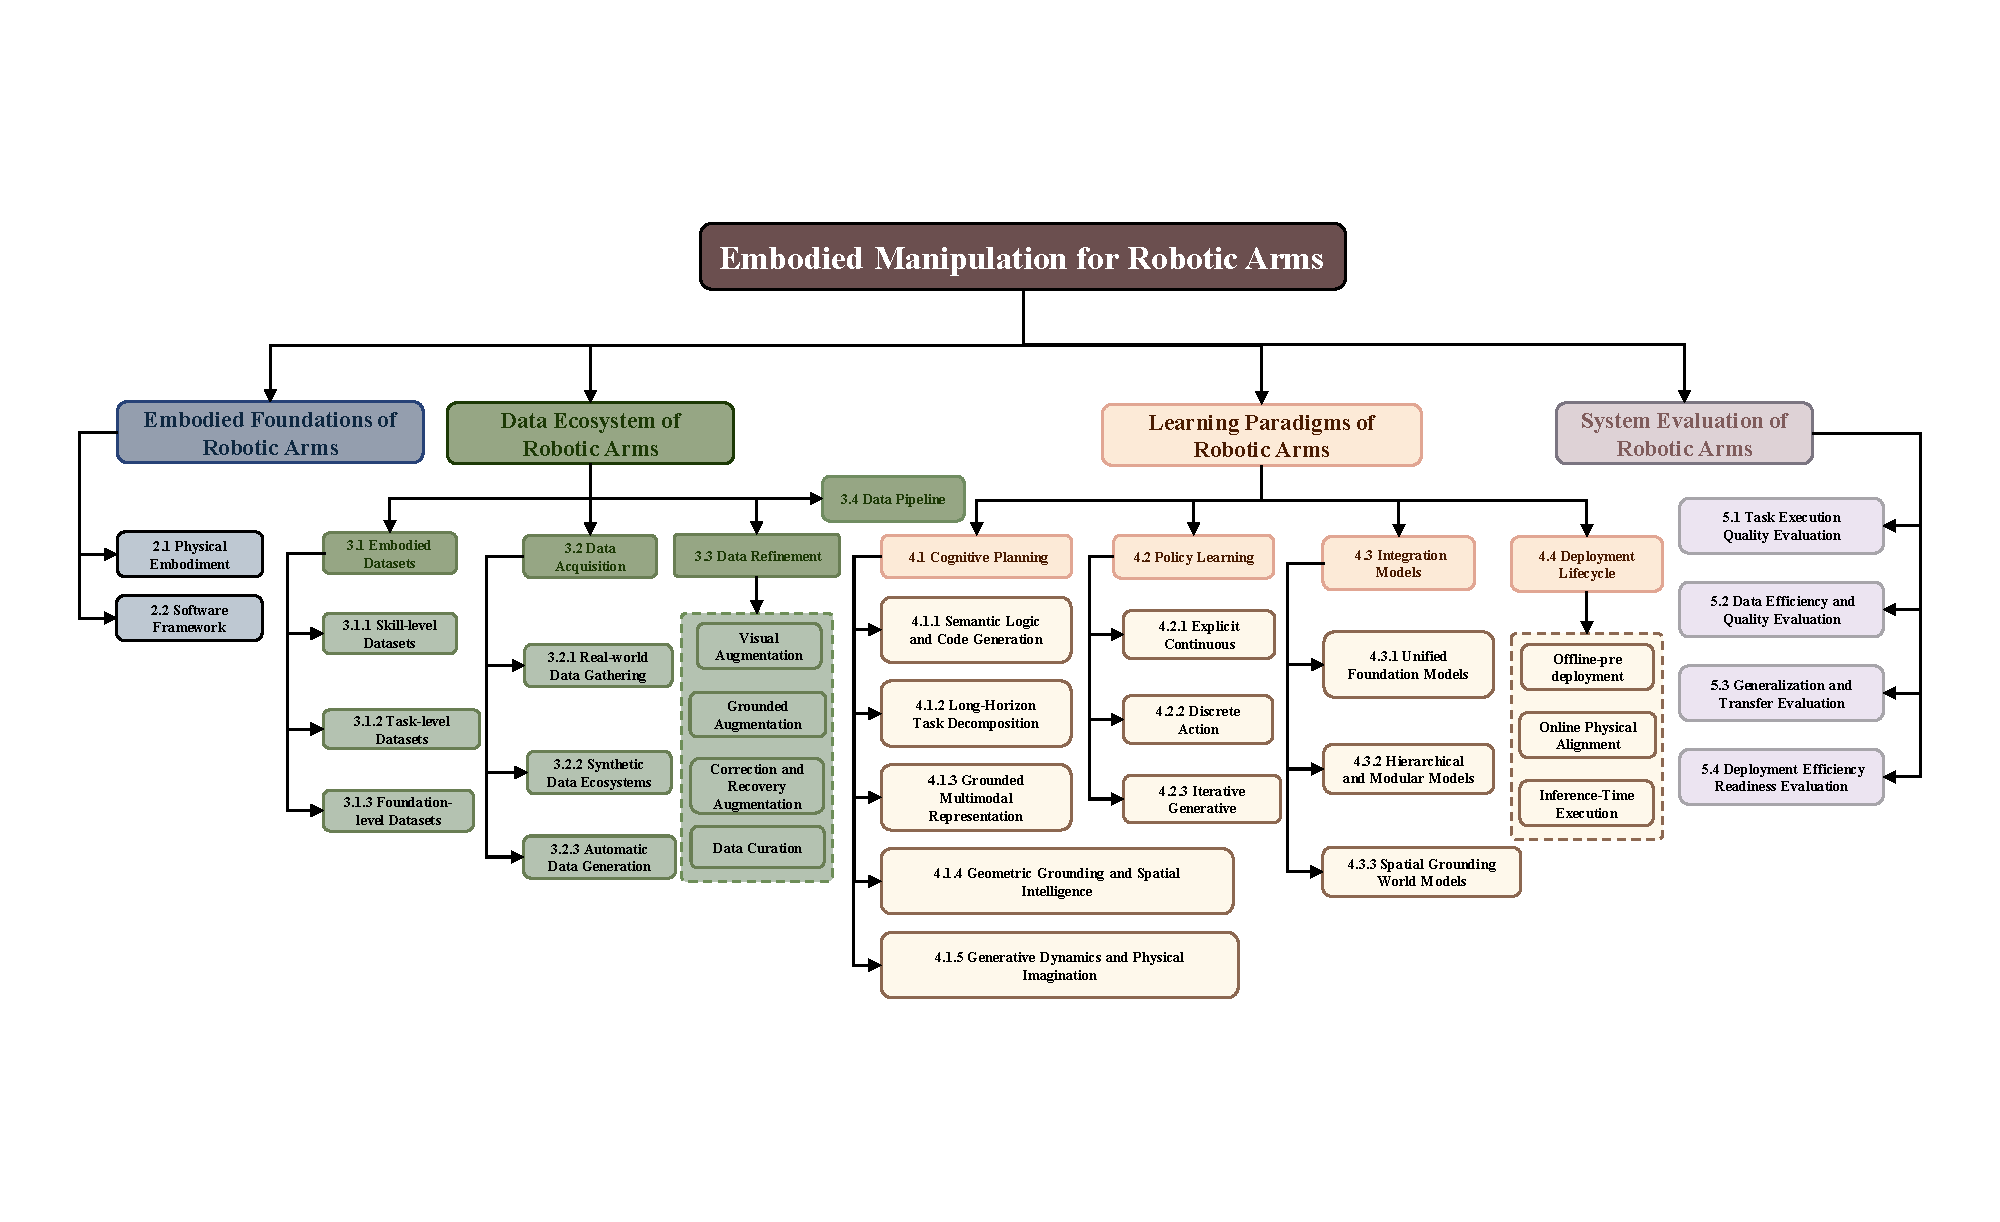
\includegraphics[width=\textwidth,trim=14cm 3.0cm 13cm 2.0cm,clip]{assets/taxonomy.pdf}
  \caption{Survey organization for embodied AI in robotic arms. The taxonomy is structured around system architecture, data ecosystem, architectural paradigms, and evaluation metrics, tracing connections from embodiment and data pipelines to cognitive planning, policy learning, integration models, deployment, and evaluation.}
  \Description{A hierarchical diagram showing the organization of the survey on embodied AI for robotic arms. The top node branches into four main pillars: system architecture, data ecosystem, architectural paradigms, and evaluation metrics. These pillars further expand into subtopics including embodied systems, dataset categories, data refinement, cognitive planning, policy learning, integration models, deployment lifecycle, and evaluation criteria. Arrows indicate conceptual dependencies across the survey structure.}\label{fig:survey_structure}
\end{figure}

The action space of a robotic system is constrained by its hardware embodiment. End-effector geometry, manipulator kinematics, and base mobility together determine what tasks a policy can physically execute. This section reviews the hardware landscape through end effectors, stationary platforms, and mobile platforms, and then examines the software stack that closes the loop from perception to actuation.

\subsection{Physical Embodiment}

The physical embodiment of a manipulation system spans three levels of abstraction (Fig.~\ref{fig:embodiment_taxonomy}): the \emph{end effector} that mediates contact, the \emph{stationary platform} that provides kinematic reach and torque bandwidth, and the \emph{mobile platform} that extends the workspace to unstructured environments.

\begin{figure}[t]
    \centering
    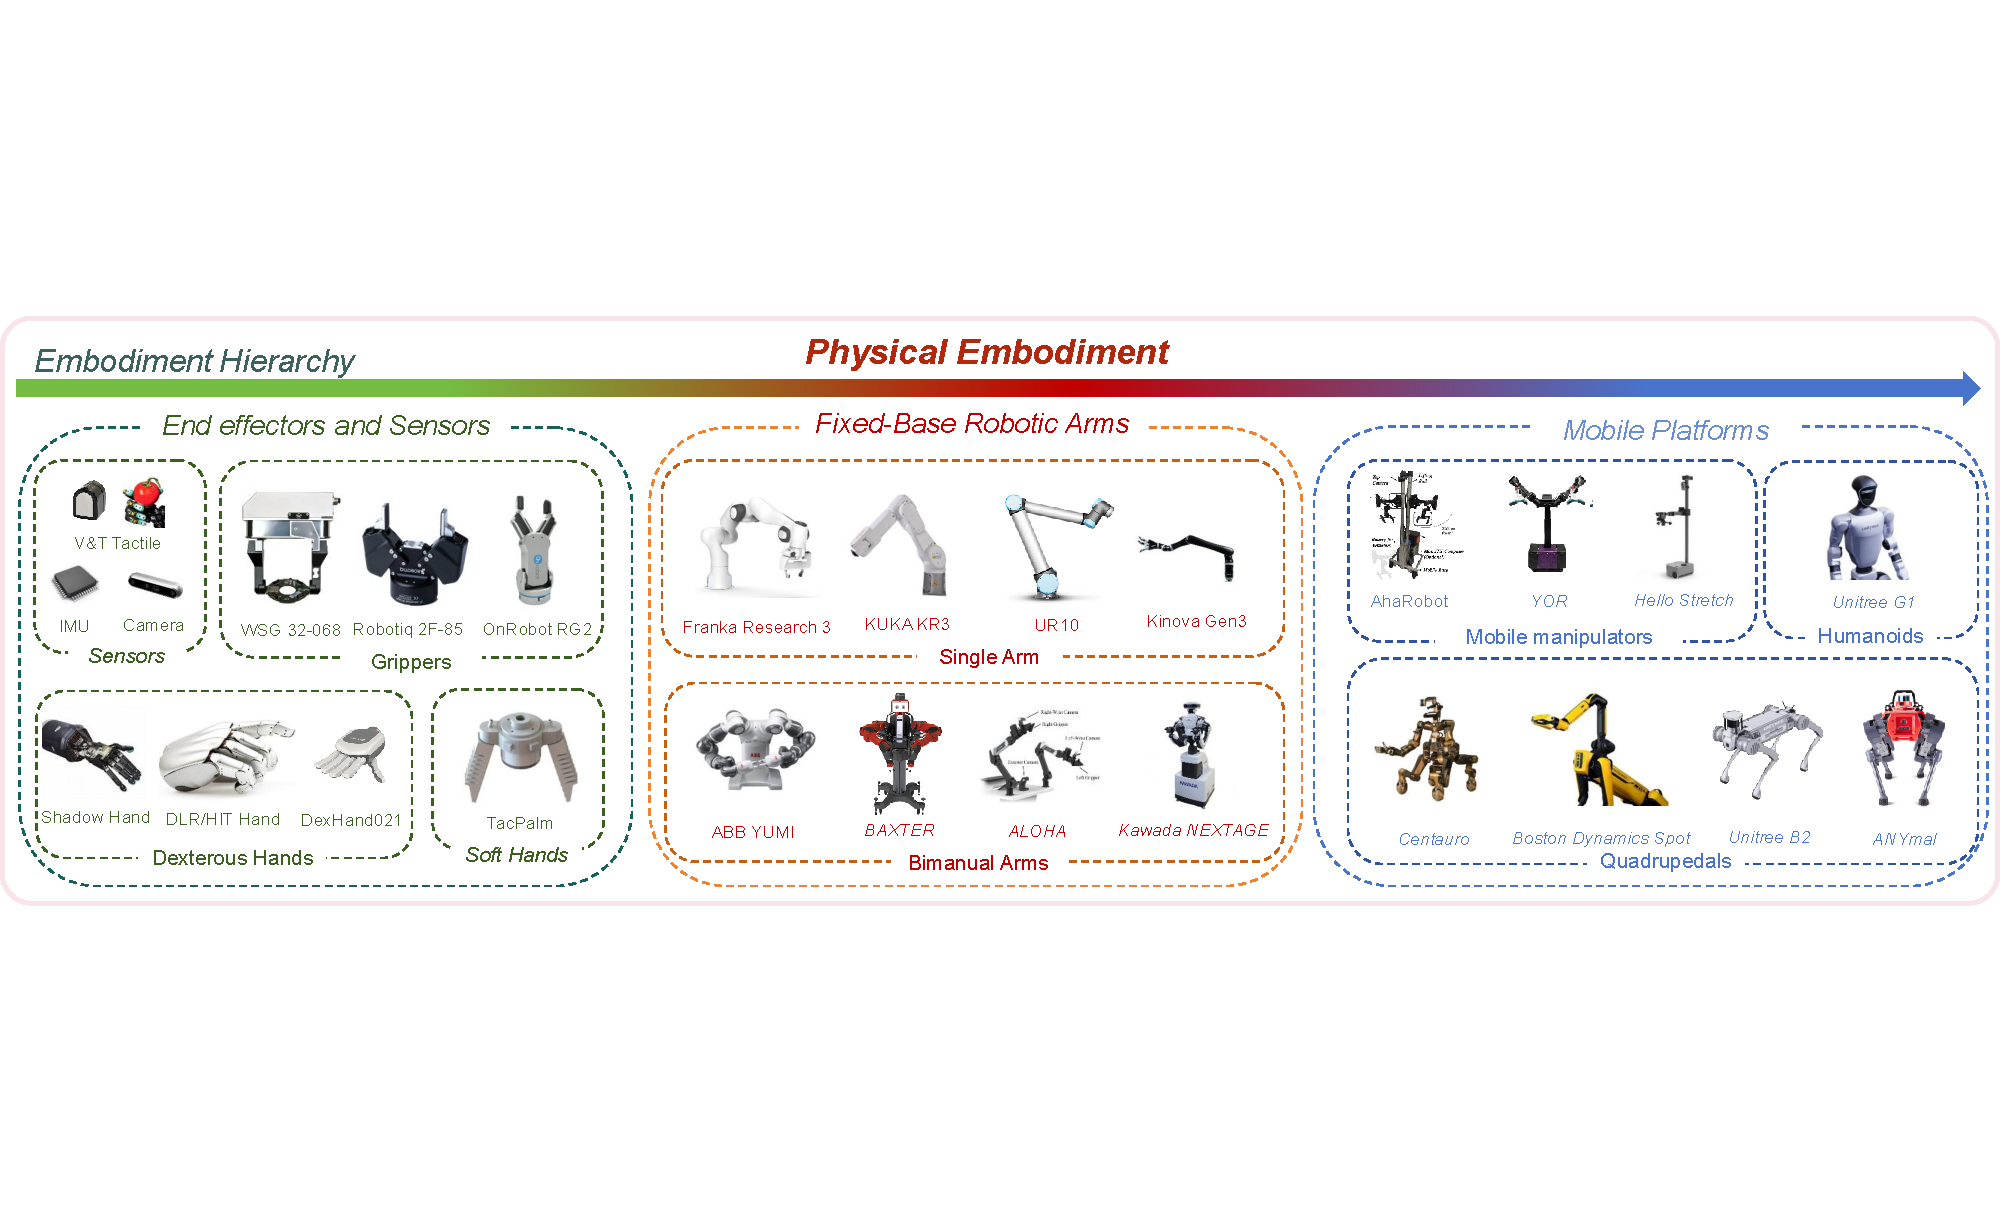
\includegraphics[width=\linewidth,trim=12cm 4.3cm 6cm 3.5cm,clip]{assets/embodiment.pdf}
    \caption{Taxonomy of physical embodiments for robotic manipulation. End effectors are classified by contact modality (jaw gripper, dexterous hand, soft hand) and sensing (vision, tactile); platforms are divided into stationary (single-arm, bimanual) and mobile (wheeled, quadrupedal, humanoid).}
    \Description{A hierarchical diagram showing the taxonomy of physical embodiments for robotic manipulation. End effectors are classified by contact modality (jaw gripper, dexterous hand, soft hand) and sensing (vision, tactile); platforms are divided into stationary (single-arm, bimanual) and mobile (wheeled, quadrupedal, humanoid).}\label{fig:embodiment_taxonomy}
\end{figure}

\subsubsection{End Effectors}\label{subsec:end_effectors}

End effectors define the contact geometry, force resolution, and sensory feedback available to the policy. Jaw grippers such as the Robotiq 2F/3F series use mechanical linkages for adaptive form closure, trading in-hand dexterity for grasp robustness. Dexterous hands---Shadow Hand (24 DoF) and Allegro Hand (16 DoF)---approximate human-level kinematics but require solving high-rank inverse kinematics under non-convex friction cone constraints. Soft hands (RBO Hand 3~\cite{Puhlmann_2022}, Festo BionicSoftHand, SpiRobs) exploit pneumatic compliance to bypass explicit force control, at the cost of state-estimation difficulty typically addressed by FEM or data-driven dynamics models. Sensing modalities determine what the policy can observe during contact. Eye-in-hand cameras (e.g., RealSense) resolve pre-contact geometry but cannot observe contact forces or slip. Tactile sensors address this gap: vision-based sensors such as GelSight~\cite{zhao2023gelsightsveltehumanfingershaped} and DIGIT embed cameras beneath deformable gel surfaces, capturing contact geometry as images, while resistive and capacitive sensors such as BioTac provide direct force and vibration measurements for slip detection and texture discrimination. The integration of visual and tactile modalities enables visuo-tactile closed-loop control for fragile objects, insertion tasks, and dynamic re-grasping.

\subsubsection{Stationary Platforms}\label{subsec:manipulators}

Fixed-base manipulators offer the highest control bandwidth and repeatability for contact-rich research. Single-arm systems such as the Franka Panda and KUKA iiwa provide joint-side torque sensing for 1\,kHz impedance control; the Kinova Gen3 adds 7-DoF continuous-rotation redundancy for null-space optimization. Bimanual setups (e.g., dual Franka Pandas, ABB YuMi) introduce closed-chain constraints requiring explicit internal-force coordination.

\subsubsection{Mobile Platforms}\label{subsec:mobile_platforms}

Mounting manipulators on mobile bases couples locomotion and manipulation into a single dynamical system. Wheeled mobile manipulators (PR2, TIAGo, Hello Robot Stretch~3) pair differential or holonomic bases with manipulation arms; controllers must reconcile non-holonomic base constraints with end-effector tracking accuracy. Quadrupedal manipulators (Spot with 6-DoF arm, Unitree GO2/B1 with 5-7 DoF arms) add terrain-adaptive stability: the controller maintains the dynamic stability margin while the arm exerts interaction forces, requiring high-frequency re-planning of foot contacts. Humanoids (Atlas: 28 DoF, Optimus Gen~2: 28+ DoF, Figure~02: 16 DoF bimanual, 1X Neo: 20 DoF, Unitree G1: 23-43 DoF) combine bipedal balance with bimanual coordination under centroidal dynamics control, where manipulation forces must be balanced against whole-body angular momentum. Payload capacity ranges from 3-5\,kg for wheeled platforms to 10-15\,kg for quadrupeds and 20-30\,kg for humanoids, with control frequencies spanning 100-1000\,Hz depending on the platform's actuation and sensing architecture.

Across these embodiment families, expanding embodiment scope increases the reachable task space but also strengthens coupling between contact, motion, and stability, shifting the bottleneck from hardware capability to real-time coordination and policy execution.

\subsection{Software Framework}

\subsubsection{Modern Robotics Middleware and Operating Systems}\label{subsec:control_middleware}

We structure the software stack into three tiers (Table~\ref{tab:framework_comparison}): the Kernel Layer (L0) for hard real-time motor control, the Transport Layer (L1) for inter-process data flow, and the System Layer (L2) for distributed orchestration.

The kernel layer (L0) centers on temporal determinism. Industrial stacks still rely on kernels such as VxWorks\footnote{\url{https://www.windriver.com/products/vxworks}} and QNX\footnote{\url{https://blackberry.qnx.com}} for bounded interrupt latency and fault isolation, while lighter RTOS options such as FreeRTOS\footnote{\url{https://www.freertos.org/}}, Zephyr\footnote{\url{https://zephyrproject.org/}}, and NuttX\footnote{\url{https://nuttx.apache.org/}} extend the same logic to resource-constrained edge devices.

The transport layer (L1) has consolidated around ROS~2 as the dominant communication backbone, with decentralized DDS replacing earlier centralized designs~\cite{macenski2022robot}. For embodied models, however, the bottleneck is increasingly not connectivity itself but the cost of moving multimodal data, which has driven low-copy or zero-copy designs such as LCM, Dora-rs, and Agnocast~\cite{huang2010lcm, zhang2026dora, ishikawa2025agnocast}.

The system layer (L2) shifts the emphasis from message passing to orchestration across robots, edge devices, clouds, and fleets. Systems such as Zenoh-Flow, Open-RMF, and FogROS2 treat deployment, routing, and compute offloading as first-class concerns, while RoboOS represents a more recent AI-native direction in which high-level multimodal planning is coupled to reusable skill libraries across heterogeneous embodiments~\cite{zenoh2024, openrmf2021, ichnowski2022fogros2, wang2025roboos}.

\begin{table*}[t]
\centering
\caption{\textbf{Three-Tier Software Architecture for Embodied Intelligence.}
\textbf{L0:} Hard real-time kernels for microsecond-level motor control determinism.
\textbf{L1:} Transport middleware for high-throughput, low-latency inter-process data flow.
\textbf{L2:} System-layer orchestration for distributed deployment, fleet management, and AI-native coordination.
\textbf{Perf.:} Interrupt/IPC latency (L0/L1) or deployment granularity (L2).}\label{tab:framework_comparison}
\renewcommand{\arraystretch}{1.2}
\setlength{\tabcolsep}{3pt}
\scriptsize

\begin{tabular}{
  p{0.11\linewidth}
  p{0.09\linewidth}
  p{0.10\linewidth}
  p{0.34\linewidth}
  p{0.10\linewidth}
  p{0.12\linewidth}
}
\toprule
\textbf{Framework} &
\textbf{Type} &
\textbf{Core Mech.} &
\textbf{Key Contribution} &
\textbf{Perf.} &
\textbf{Scope} \\
\midrule

\multicolumn{6}{c}{\textbf{L0: Kernel Layer --- Hard Real-Time Execution}} \\
\midrule

\textbf{VxWorks} &
Monolithic RTOS &
Priority Preemptive &
Industry-standard deterministic kernel; bounded interrupt latency via priority-based preemptive scheduling for synchronous multi-axis servo control in aerospace and industrial automation. &
$<$10\,$\mu$s &
Industrial / Aerospace \\

\textbf{QNX} &
Microkernel &
Spatial Isolation &
Microkernel architecture isolating drivers and protocols into independent user-space memory segments; memory faults in peripherals cannot crash the core scheduling loop. POSIX-certified. &
$<$5\,$\mu$s &
Safety-critical / Automotive \\

\textbf{Zephyr} &
Modular RTOS &
Device Tree + SMP &
Linux Foundation governed; scalable device tree architecture with native SMP support; enforces strict memory domain protection even on microcontrollers without hardware MMUs. &
$<$20\,$\mu$s &
MCU / Robotic Edge \\

\midrule
\multicolumn{6}{c}{\textbf{L1: Transport Layer --- High-Throughput Data Flow}} \\
\midrule

\textbf{ROS~2}~\cite{macenski2022robot} &
Decentralized &
DDS (RTPS) &
Replaced ROS~1's centralized Master with decentralized DDS\@; granular QoS policies for reliability, deadline, and liveliness. Current \emph{de facto} communication backbone for the robotics community. &
1--10\,ms &
General Robotics \\

\textbf{LCM}~\cite{huang2010lcm} &
Masterless &
UDP Multicast &
Lightweight marshalling with minimal serialization overhead; masterless UDP multicast eliminates broker bottleneck for high-frequency legged locomotion control loops ($>$1\,kHz). &
$<$1\,ms &
Legged Robots \\

\textbf{Dora-rs}~\cite{zhang2026dora} &
Dataflow &
Apache Arrow &
Rust-based dataflow framework integrating Apache Arrow columnar format for zero-copy shared memory; eliminates serialization jitter between Python deep learning inference and Rust execution loops. &
$<$50\,$\mu$s (IPC) &
Low-latency AI \\

\textbf{Agnocast}~\cite{ishikawa2025agnocast} &
Zero-Copy IPC &
Shared Memory &
True zero-copy pub/sub for \emph{all} ROS~2 message types including dynamically-sized payloads (PointCloud2, Image); rclcpp-compatible. 25\% worst-case latency reduction on Autoware pipelines. &
Const.\ overhead &
ROS~2 Ecosystem \\

\midrule
\multicolumn{6}{c}{\textbf{L2: System Layer --- Distributed Orchestration \& AI-Native OS}} \\
\midrule

\textbf{Zenoh}~\cite{zenoh2024} &
DAG Orchestration &
Zenoh Protocol &
Declarative dataflow framework defining robotic pipelines as DAGs; automatically deploys and routes execution nodes across MCUs, edge GPUs, and cloud servers via the Zenoh protocol. &
Edge-to-Cloud &
Distributed Systems \\

\textbf{FogROS2}~\cite{ichnowski2022fogros2} &
Cloud Extension &
ROS~2 Graph &
Natively extends ROS~2 computational graph into cloud environments; robots offload latency-tolerant semantic reasoning to cloud while maintaining high-frequency reactive control on local edge. &
Hybrid &
Robot-as-a-Service \\

\textbf{RoboOS}~\cite{wang2025roboos} &
Brain--Cerebellum &
MLLM + Skill Lib &
Hierarchical architecture: MLLM-based embodied brain for global perception, task planning, and multi-agent scheduling; modular cerebellum skill library for low-level motor execution. Cross-embodiment adaptability. &
Agentic Logic &
Multi-Agent \\

\bottomrule
\end{tabular}
\end{table*}

\subsubsection{Low-level Motion Planning and Control}

While middleware provides the communication infrastructure, the low-level motion planning and control layer turns task-space intents into physically executable joint commands. Its central burden is to satisfy several coupled constraints at once: mapping between operational and joint space, compensating nonlinear rigid-body dynamics, respecting joint and collision limits, and remaining stable under external contact~\cite{sicilianoSpringerHandbookRobotics2016}. For this reason, modern embodied systems increasingly rely on optimization-based controllers, especially model predictive control and whole-body control, which treat tracking, feasibility, and safety as a single constrained problem updated at control rate rather than as separate planning and servo stages~\cite{schulman2014optimizing}.

In manipulation, contact behavior is as important as free-space accuracy. Impedance control remains a standard mechanism for shaping compliant interaction during assembly, tool use, and human---robot collaboration, because it lets the robot trade stiffness for robustness instead of treating every deviation as pure tracking error~\cite{hogan1985impedance}. In practice, the effectiveness of MPC, WBC, and impedance control still depends on L0-level temporal determinism: timing jitter in the execution loop can destabilize high-frequency feedback long before perception or learning becomes the limiting factor.

Together, hardware embodiment and the software stack define the physical and computational constraints under which any learned policy must operate. The next question is what data is required to learn effectively under these constraints, and how that data should be structured, collected, and scaled.

\section{Data Ecosystem of Robotic Arms}\label{sec:embodiment_dataset}

Large-scale manipulation research depends on both the data regimes available to learning systems and the infrastructures that produce them. This chapter is therefore organized along two complementary views: \S\ref{sec:eai_datasets} characterizes the knowledge carried by embodied datasets, while \S\ref{sec:data_acquisition}--\ref{sec:data_factories_robotic_arms} examine the production stack that collects, generates, refines, and integrates that knowledge at scale.

\subsection{Embodied Datasets}\label{sec:eai_datasets}

Embodied datasets provide the foundation for manipulation learning. Their key differences lie in the type of supervision and knowledge they contribute to downstream systems. We therefore organize existing datasets into three tiers according to the dominant knowledge regime they expose (see Fig.~\ref{fig:evolution} and Tables~\ref{tab:grasping_datasets}--\ref{tab:foundation_datasets}).

\textbf{Skill-level datasets} ($\mathcal{K}_1$) densely sample local interaction phenomena such as grasp geometry, contact patterns, and material response. Supervision targets single atomic actions: whether a grasp succeeds, how a push affects object motion, or which contact forces arise during insertion. Success is typically evaluated per action rather than per task. \textbf{Task-level datasets} ($\mathcal{K}_2$) shift supervision to multi-step sequences indexed by natural language instructions. A trajectory is judged by whether the full instruction is completed rather than whether each individual action succeeds. This requires learning not only how individual skills work, but when and in what order to invoke them. \textbf{Foundation-level datasets} ($\mathcal{K}_3$) shift supervision again, now targeting transfer across robot morphologies. The primary objective becomes whether a policy generalizes to unseen embodiments under heterogeneous sensors and action spaces.

Taken together, these tiers describe an ordered progression from local interaction grounding to task composition and then to cross-embodiment generalization. We use the shorthand $\mathcal{K}_i \approx \mathcal{K}_{i-1} \oplus \mathcal{D}_i$ to denote that each tier augments the previous one with new supervision, diversity, and transfer demands.

\subsubsection{Skill-level Datasets}\label{sec:skill_datasets_narrative}

Skill-level datasets densely sample atomic motor primitives and their local interaction dynamics (Table~\ref{tab:grasping_datasets}). 
Early grasping benchmarks such as Cornell~\cite{lenz2014deep} represented graspable regions as 2D oriented rectangles, limiting coverage to top-down parallel-jaw approaches. 
Dex-Net 2.0~\cite{mahler2017dex} addressed data scarcity through analytical synthesis based on force-closure metrics, generating millions of grasp labels. 
GraspNet-1B~\cite{fang2020graspnet} scaled real-world 6-DoF grasp annotation to 1.2 billion grasps across cluttered scenes; 
GraspClutter6D~\cite{back2025graspclutter6d} further increased clutter density and annotation coverage. 
Multi-fingered systems with $>$20 DoF extend skill-level supervision from parallel-jaw grasping to dexterous, cluttered, and partially occluded contact regimes: 
DexGraspNet 2.0~\cite{zhang2024dexgraspnet20learninggenerative} provides approximately 427M synthetic grasps with 90.7\% real-world success via diffusion-based synthesis, 
and Dex1B~\cite{ye2025dex1b} scales to one billion grasps. Tactile modalities complement vision at this level; 
T-DEX~\cite{guzey2023tdex} shows that self-supervised pre-training on 2.5 hours of unstructured tactile play data outperforms vision-only baselines by 1.7$\times$ on five dexterous tasks, capturing slip and in-hand reorientation signals that are unobservable through vision alone. 
Beyond grasping, Omnipush~\cite{bauza2021omnipush} quantifies planar pushing dynamics across 250 objects, 
PartNet-Mobility~\cite{xiang2020sapien} provides part-level interaction data for articulated objects, 
and FurnitureBench~\cite{heo2023furniturebench} supplies over 5,000 teleoperated trajectories for precision assembly with a paired simulator. 
Recent datasets also begin to couple local grasp affordances with language, bridging low-level grasp supervision and instruction-conditioned manipulation; these are discussed alongside task-level data in \S\ref{sec:task_datasets_narrative}.

\begin{table*}[t]
\centering
\caption{\textbf{Chronological Overview of Skill-level Datasets.} Evolution reflects the shift from planar grasping rectangles to dense 6-DoF poses, dexterous hands, language-grounded reasoning, and diverse motor primitives (pushing, articulation, deformable manipulation, assembly). Note the scarcity of real-world data for non-grasping primitives.}\label{tab:grasping_datasets}
\resizebox{\textwidth}{!}{%
\begin{tabular}{l c c c c c c c c}
\toprule
\textbf{Dataset} & \textbf{Year} & \textbf{Skill Type} & \textbf{Scene Complexity} & \textbf{Objects} & \textbf{Domain} & \textbf{Scale (Size)} & \textbf{Modality} & \textbf{Lang.} \\
\midrule
\multicolumn{9}{c}{\textbf{Early Geometric Grasping}} \\
\midrule
\textbf{Cornell}~\cite{lenz2014deep} & 2011 & Rect.\ Grasp (2D) & Single Object & 240 & Real & 1k imgs & RGB-D & $\times$ \\
\textbf{Dex-Net 2.0}~\cite{mahler2017dex} & 2017 & Parallel-Jaw Grasp & Single Object & 1.5k & Sim & 6.7M grasps & Depth & $\times$ \\
\textbf{Jacquard}~\cite{depierre2018jacquard} & 2018 & Rect.\ Grasp (2D) & Single Object & 11k & Sim & 54k imgs (1.1M grasps) & RGB-D & $\times$ \\
\midrule
\multicolumn{9}{c}{\textbf{Dense 6-DoF Grasping}} \\
\midrule
\textbf{GraspNet-1B}~\cite{fang2020graspnet} & 2020 & 6-DoF Grasp & Heavy Clutter & 88 & Real & 97k imgs (1.2B grasps) & RGB-D & $\times$ \\
\textbf{ACRONYM}~\cite{eppner2020acronym} & 2021 & 6-DoF Grasp & Multi-Object & 8,872 & Sim & 17.7M grasps & RGB-D & $\times$ \\
\textbf{GraspClutter6D}~\cite{back2025graspclutter6d} & 2025 & 6-DoF Grasp & Cluttered & 200 & Real & 52k imgs (9.3B grasps) & RGB-D & $\times$ \\
\midrule
\multicolumn{9}{c}{\textbf{Dexterous Grasping}} \\
\midrule
\textbf{DexGraspNet}~\cite{wang2023dexgraspnetlargescaleroboticdexterous} & 2023 & Dexterous Grasp & Single Object & 5,355 & Sim & 1.32M grasps & Point Cloud & $\times$ \\
\textbf{DexGraspNet 2.0}~\cite{zhang2024dexgraspnet20learninggenerative} & 2024 & Dexterous Grasp & Multi-Object & 5,355 & Sim & 427M grasps & Point Cloud & $\times$ \\
\textbf{Dex1B}~\cite{ye2025dex1b} & 2025 & Dexterous Grasp & Single Object & 1M & Sim & 1B grasps & Point Cloud & $\times$ \\
\midrule
\multicolumn{9}{c}{\textbf{Language-Grounded Grasping}} \\
\midrule
\textbf{OCID-VLG}~\cite{tziafas2023ocidvlg} & 2023 & Rect.\ Grasp & Multi-Object & 89 & Real & 75k grasps & RGB-D & $\checkmark$ \\
\textbf{Grasp-Anything}~\cite{vuong2023graspanything} & 2023 & Rect.\ Grasp + Push & Multi-Object & 3M & Syn & 1M imgs (600M grasps) & RGB & $\checkmark$ \\
\textbf{ReasoningGrasp}~\cite{jin2024reasoninggrasp} & 2024 & 6-DoF Grasp & Multi-Object & 64 & Real & 99M grasps & RGB-D & $\checkmark$ \\
\midrule
\multicolumn{9}{c}{\textbf{Diverse Motor Primitives (Non-Grasping)}} \\
\midrule
\textbf{Omnipush}~\cite{bauza2021omnipush} & 2019 & Pushing (Planar) & Single Object & 250 & Real & 62.5k pushes & RGB-D & $\times$ \\
\textbf{PartNet-Mobility}~\cite{xiang2020sapien} & 2020 & Articulated (Open/Close) & Single Object & 2,346 models & Sim & 2,346 articulated assets & 3D / PC & $\times$ \\
\textbf{FlowBot3D}~\cite{ben2022flowbot3d} & 2022 & Articulated (Flow) & Cluttered & 1k+ & Sim & Per-point 3D flow fields & 3D / PC & $\times$ \\
\textbf{FurnitureBench}~\cite{heo2023furniturebench} & 2023 & Assembly (Precise) & Tabletop & Furniture & Sim+Real & 5.1k demos (220 hrs) & RGB & $\times$ \\
\textbf{UniFolding}~\cite{xue2023unifolding} & 2023 & Deformable (Folding) & Multi-Object & Garments & Sim+Real & Sample-efficient ($<$1k) & RGB-D & $\times$ \\
\bottomrule
\end{tabular}
}
\end{table*}

\subsubsection{Task-level Datasets}\label{sec:task_datasets_narrative}

Task-level datasets bind atomic motor primitives into temporally extended, instruction-aligned trajectories. Where skill-level data answers \emph{how} a single action succeeds, task-level data answers \emph{what sequence of actions} completes a goal (Table~\ref{tab:real_world_tasks}).

Early fleet-scale collection established that data volume improves multi-task success rates. MT-Opt~\cite{kalashnikov2021mt} collected 800k trajectories through autonomous exploration, but these lacked language grounding and indexed actions by task ID rather than natural instructions. The introduction of language-conditioned trajectories shifted the field substantially. BC-Z~\cite{jang2022bc} paired 26k trajectories with 100 semantic verbs, demonstrating that language supervision enables generalization across task descriptions. RT-1 Dataset~\cite{brohan2023rt1} scaled this paradigm to 130k trajectories spanning 700+ instructions on the Everyday Robot platform, enabling the first instruction-following policies that generalize across diverse task descriptions.

These early datasets were collected in one or two institutional kitchens, limiting environmental diversity. Distributed collection addressed this bottleneck. BridgeData V2~\cite{walke2024bridgedatav2} aggregated 60k trajectories across 24 scenes via multi-site collection, and DROID~\cite{khazatsky2024droid} coordinated 18 institutions to collect 76k trajectories in 564 distinct scenes with calibrated extrinsics. Dobb-E~\cite{shafiullah2023bringing} reduced hardware requirements by mounting an iPhone on a Stretch robot, accessing 22 domestic environments. Beyond visual diversity, FMB~\cite{fu2025fmb} emphasized physical grounding through rigorous force-torque calibration across 22k contact-rich assembly trajectories.

More recently, datasets have begun to incorporate failure supervision alongside successful demonstrations. RoboMIND~\cite{wu2025robomind} collected 107k trajectories across 4 robots with 5,000 failure demonstrations annotated with explicit error causes, enabling models to learn recovery behaviors. RoboMIND 2.0~\cite{hou2026robomind20} further scales to 310k trajectories across 6 robots and 739 tasks, expanding cross-embodiment coverage while maintaining failure-aware supervision.

\begin{table*}[t] 
\centering
\caption{Taxonomy of Task-level Embodied Datasets: Real-world Physical Trajectories.}\label{tab:real_world_tasks}
\footnotesize 
\setlength{\tabcolsep}{2.5pt} 
\resizebox{\textwidth}{!}{ 
\begin{tabular}{lcccccccc}
\toprule
\textbf{Dataset} & \textbf{Year} & \textbf{\# Traj.} & \textbf{Verbs} & \textbf{Scenes} & \textbf{Lang.} & \textbf{Calib.} & \textbf{Robot} & \textbf{Collection} \\
\midrule
MIME~\cite{sharma2018mime} & 2018 & 8.3k & 20 & 1 & $\times$ & $\times$ & Baxter & Teleop. \\
RoboTurk~\cite{mandlekar2018roboturk} & 2018 & 2.1k & 2 & 1 & $\times$ & $\times$ & Panda & Teleop. \\
MT-Opt~\cite{kalashnikov2021mt} & 2021 & 800k & 2 & 1 & $\times$ & $\times$ & Google Arm & Mixed \\
BC-Z~\cite{jang2022bc} & 2021 & 26k & 100 & 1 & $\checkmark$ & $\times$ & EDR & Teleop. \\
BridgeData V1~\cite{ebert2021bridgedata} & 2022 & 7.2k & 4 & 12 & $\checkmark$ & $\times$ & WidowX & Teleop. \\
RT-1 Dataset~\cite{brohan2023rt1} & 2022 & 130k & 700+ & 2 & $\checkmark$ & $\times$ & EDR & Teleop. \\
RoboSet~\cite{bharadhwaj2023roboagent} & 2023 & 98.5k & 12 & 11 & $\checkmark$ & $\times$ & Panda & H/S Hybrid \\
Dobb-E~\cite{shafiullah2023bringing} & 2023 & 1.5k & 109 & 22 & $\times$ & $\times$ & Stretch & iPhone \\
BridgeData V2~\cite{walke2024bridgedatav2} & 2024 & 60k & 82 & 24 & $\checkmark$ & $\times$ & WidowX & H/S Hybrid \\
DROID~\cite{khazatsky2024droid} & 2024 & 76k & 50+ & 564 & $\checkmark$ & $\checkmark$ & Panda & Teleop. \\
FMB~\cite{fu2025fmb} & 2025 & 22k & 10 & 1 & $\checkmark$ & $\checkmark$ & Panda & Mixed \\
RoboMIND~\cite{wu2025robomind} & 2025 & 107k & 479 & \- & $\checkmark$ & $\times$ & 4 types & Teleop. \\
RoboMIND 2.0~\cite{hou2026robomind20} & 2026 & 310k & 739 & \- & $\checkmark$ & $\checkmark$ & 6 types & Teleop. \\
\bottomrule
\end{tabular}
}
\end{table*}

\subsubsection{Foundation-level Datasets}\label{sec:foundation_datasets}

Foundation-level datasets aggregate experience across heterogeneous robot morphologies under standardized observation and action protocols (Table~\ref{tab:foundation_datasets}), supporting cross-embodiment transfer by exposing models to generalized transition dynamics across platforms. RoboNet~\cite{dasari2020robonet} initiated multi-institutional data sharing with 162k trajectories across seven robot platforms. OXE~\cite{padalkar2023open} scaled this to over one million trajectories from 22 morphologies, standardized via the RLDS protocol, enabling the first cross-embodiment foundation model training experiments. Aggregating heterogeneous data also introduces observation misalignment across camera configurations and sensor setups. ARIO~\cite{wang2024ario} addresses this with approximately 3 million episodes featuring synchronized multi-view timestamps, and RH-20T~\cite{fang2023rh} extends the sensory scope beyond vision by integrating force-torque and audio signals across 110k sequences for contact-rich manipulation. More recently, AgiBot World Beta~\cite{agibot2025} provides over one million trajectories ($\sim$43.8 TB) collected from 100+ humanoid robots for bimanual coordination and 6-DoF dexterous manipulation. Complementing robot-centric data, Ego-Exo4D~\cite{grauman2024egoexo4d} provides 740 hours of synchronized first- and third-person human video across 8 activity domains, linking abundant human demonstration footage with the exocentric viewpoints typical of robotic systems.

\begin{table*}[t!]
\centering
\caption{Foundation-level Datasets for Cross-Embodiment Manipulation.
\# Traj.\,=\,trajectory count;
\# Embod.\,=\,distinct robot platforms/configurations when explicitly reported;
Embod.\ Types: S\,=\,single-arm, B\,=\,bimanual, M\,=\,mobile manipulator, H\,=\,humanoid;
Modalities beyond RGB: D\,=\,depth, F\,=\,force/torque, A\,=\,audio;
Lang.\,=\,language supervision;
Action: EE\,=\,end-effector, Emb.\,=\,embodiment-specific, WB\,=\,whole-body;
Alignment: how cross-embodiment differences are reconciled.}
\label{tab:foundation_datasets}
\renewcommand{\arraystretch}{1.15}
\setlength{\tabcolsep}{2.5pt}
\scriptsize
\begin{tabular}{lccclclccll}
\toprule
\textbf{Dataset} & \textbf{Year} & \textbf{\# Traj.} & \textbf{\# Embod.} & \textbf{Types} & \textbf{Source} & \textbf{Modalities} & \textbf{Lang.} & \textbf{Action} & \textbf{Alignment} & \textbf{Schema} \\
\midrule
RoboNet~\cite{dasari2020robonet} & 2019 & 162k & 7 & S & Scripted & RGB & $\times$ & EE & Interface-level & Custom \\
RH-20T~\cite{fang2023rh} & 2023 & 110k & 7 & S & Teleop & RGB, D, F, A & $\checkmark$ & Emb. & Calibration-level & Custom \\
OXE~\cite{padalkar2023open} & 2023 & 1M+ & 22 & S, B, M & Aggregated & RGB (varied) & $\checkmark$ & EE & Schema-level & RLDS \\
ARIO~\cite{wang2024ario} & 2024 & 3M & -- & S, B, M & Aggregated (Real+Sim) & RGB, D & $\checkmark$ & Emb. & Temporal & Unified \\
AgiBot World~\cite{agibot2025} & 2025 & 1M+ & 100+ & B, H & Teleop & RGB, D, F & $\checkmark$ & WB & Pipeline-level & Custom \\
\bottomrule
\end{tabular}
\end{table*}

\subsection{Data Acquisition}\label{sec:data_acquisition}

The dataset taxonomy above establishes what knowledge each tier provides; this subsection examines how that knowledge is acquired in practice. Three complementary channels supply training corpora for manipulation learning: real-world gathering captures the physical fidelity that no simulator fully reproduces, simulation ecosystems provide scalable and controllable environments for generating diverse experience, and automatic data generation amplifies limited seed demonstrations through programmatic or generative means. Together, these channels form the production stack that populates the skill-level, task-level, and foundation-level regimes described in \S\ref{sec:eai_datasets}.

\subsubsection{Real-world Data Gathering}\label{sec:real_acquisition}

Real-world data acquisition has evolved along four concurrent lines. MIME~\cite{sharma2018mime} provided large-scale paired human-robot demonstrations, and RoboTurk~\cite{mandlekar2018roboturk} showed that remote operators could be coordinated for distributed collection. Low-cost teleoperation matured through ALOHA~\cite{zhao2023learning, fu2024mobile}, which reduced the hardware barrier for bimanual and mobile whole-body data collection, and AnyTeleop~\cite{qin2024anyteleop}, which lowered cross-platform retargeting overhead. Distributed collection scaled through DROID~\cite{khazatsky2024droid}, which coordinated 18 institutions to gather 76k trajectories across 564 scenes with standardized protocols. Robot-decoupled demonstration emerged through portable systems: UMI~\cite{chi2024umi} enabled in-the-wild collection with handheld grippers and consumer cameras, DexCap~\cite{wang2024dexcap} extended this to dexterous capture through wearable motion tracking, and AirExo-2~\cite{fang2025airexo2} supported human-to-robot adaptation via image inpainting and differentiable rendering. For humanoid robots, OmniH2O~\cite{he2025omnih2o} addresses the structural mismatch between human and robotic skeletons through massively parallel motion retargeting in simulation, enabling human demonstrations to be converted into whole-body control data. Autonomy-assisted collection began with RoboCat~\cite{bousmalis2023robocat}, which combined self-improving loops with selective human takeover, and scaled to system-level orchestration through AutoRT~\cite{gdm2024autort}, which used foundation models to coordinate robot fleets for diverse real-world task execution under safety constraints. Two complementary trends have emerged: data sources increasingly decouple from robot presence through egocentric human video (EgoMimic~\cite{kareer2025egomimic}, AoE~\cite{yang2026aoe}), while data factories increasingly automate the collection-failure-improvement cycle with minimal human supervision~\cite{mendonca2025continually}. The correction mechanisms that support such loops are discussed in \S\ref{sec:correction_recovery}, and their pipeline-level industrial instantiations in \S\ref{sec:data_factories_robotic_arms}. 

\subsubsection{Simulation Data Ecosystems}\label{sec:simulation_infrastructure}

Simulation in manipulation is now organized around a few reusable ecosystems with distinct data strengths (Table~\ref{tab:sim_classification}). The three most influential are MuJoCo, which prioritizes stable contact and controller-facing dynamics; SAPIEN, which centers articulated-object interaction and part semantics; and NVIDIA Isaac, which emphasizes GPU-parallel synthesis at scale. Specialized platforms remain important when the target is a narrower benchmark, a particular task family, or a physical regime that the dominant ecosystems do not cover well.

\begin{table*}[t]
\centering
\caption{\textbf{Landscape of Simulation Infrastructures for large embodied models} We re-categorize platforms into the three dominant ecosystems driving modern manipulation research (MuJoCo, SAPIEN, Isaac) and specialized platforms serving as functional baselines. This taxonomy highlights the transition from task-specific simulators to comprehensive generative data factories.}\label{tab:sim_classification}
\resizebox{\textwidth}{!}{%
\begin{tabular}{@{}l p{4.2cm} p{5.8cm} p{5.5cm}@{}}
\toprule
\textbf{Simulator} & \textbf{Features} & \textbf{Capabilities \& Modalities} & \textbf{Key Benchmarks \& Datasets} \\
\midrule
\multicolumn{4}{c}{\textbf{\textbf{I. The Core Simulation Ecosystems}}} \\
\midrule
\addlinespace[0.5ex]
\textbf{MuJoCo} & Stable analytic contact solver; MJX hardware acceleration (TPU/GPU); Unified differentiable dynamics. & \textbf{Physics-Aligned Data}: Artifact-free trajectories for fine-grained motor control. 

\textbf{Modalities: Proprioception (Joint states), Contact forces, Kinematics, RGB.} & \textbf{RoboCasa}~\cite{nasiriany2024robocasa}, \textbf{LIBERO}~\cite{liu2023libero}, \textbf{RoboCerebra}~\cite{han2025robocerebra}, \textbf{BiGym}~\cite{chernyadev2024bigym}, \textbf{Meta-World}~\cite{yu2021meta} \\ \addlinespace

\textbf{Isaac Suite} & Massive GPU parallelism (PhysX5);RTX-enabled neural rendering; LLM-driven generative synthesis. & \textbf{Generative \& Scalable Data}: Billion-scale synthetic distributions and high-DoF control.

\textbf{Modalities: RGB-D, LiDAR, Segmentation, Bounding boxes, Force/Torque, Event camera.} & \textbf{Isaac Lab}~\cite{mittal2023orbit}, \textbf{DexGraspNet}~\cite{wang2023dexgraspnetlargescaleroboticdexterous}, \textbf{FurnitureBench}~\cite{heo2023furniturebench}, \textbf{Factory}~\cite{narang2022factory}, \textbf{BiDexHands}~\cite{chen2022bidexhands} \\ \addlinespace

\textbf{SAPIEN} & High-fidelity articulated dynamics; Part-level mobility (PartNet); Parallelized Vulkan rendering. & \textbf{Semantic Interaction Data}: Interactions across articulated categories and part-level reasoning. 

\textbf{Modalities: RGB-D, Semantic/Instance masks, Contact forces, Articulated object states.} & \textbf{ManiSkill3}~\cite{tao2025maniskill3}, \textbf{SIMPLER}~\cite{li2025simpler}, \textbf{RoboTwin 2.0}~\cite{chen2025robotwin2}, \textbf{RoboFactory}~\cite{qin2025robofactory} \\ \addlinespace

\midrule

\multicolumn{4}{c}{\textbf{\textbf{II\@. Specialized Task Platforms}}} \\
\midrule
\addlinespace[0.5ex]
\textbf{PyBullet / CoppeliaSim} & Lightweight legacy physics; Stable IK solvers; Broad hardware and ROS abstraction. & \textbf{Algorithmic Baseline Data}: Logic planning and action primitives. 

\textbf{Modalities: RGB-D, Joint states, Contact forces, Proximity sensors, Force/Torque.} & \textbf{CALVIN}~\cite{mees2022calvin}, \textbf{RLBench}~\cite{james2020rlbench}, \textbf{Ravens}~\cite{zhang2019raven} \\ \addlinespace

\textbf{Habitat / AI2-THOR} & Procedural indoor scene generation; High-throughput visual navigation kernels. & \textbf{Embodied Navigation Data}: Semantic search and indoor reasoning. 

\textbf{Modalities: RGB-D, Semantic/Instance segmentation, Object states, Agent pose, Audio.} & \textbf{OpenEQA}~\cite{majumdar2024openeqa}, \textbf{ALFRED}~\cite{shridhar2020alfred} \\ \addlinespace

\textbf{SoftGym / Genesis} & Unified MPM/FEM/PBD solvers; Differentiable multi-physics; Automated program generation. & \textbf{Generative Multi-Physics Data}: Coupled interactions (rigid/soft/fluid). 

\textbf{Modalities: RGB-D, Proprioceptive haptics, Particle states, Differentiable gradients.} & \textbf{ClothFunnels}~\cite{canberk2022clothfunnels}, \textbf{Difftaichi}~\cite{hu2020difftaichi} \\
\bottomrule
\end{tabular}%
}
\end{table*}

\textbf{MuJoCo}~\cite{todorov2012mujoco} remains the reference ecosystem when the priority is contact stability together with controller-oriented evaluation. Its enduring role comes from a useful trade-off: the simulator is lightweight enough for rapid benchmarking while remaining faithful enough for fine-grained motor-control studies. Meta-World~\cite{yu2021meta} established the canonical state-based multi-task setting, and later suites such as LIBERO~\cite{liu2023libero} and RoboCasa~\cite{nasiriany2024robocasa} broadened the distribution toward lifelong-learning curricula and richer household scenes. In the foundation-model era, MJX and MuJoCo Playground extend the same ecosystem toward larger-batch rollouts, differentiable simulation, and stronger sim-to-real diagnostics~\cite{deepmind2025playground}.

\textbf{SAPIEN}~\cite{xiang2020sapien} addresses a different need: interaction with articulated objects whose kinematic structure must be represented explicitly. It couples physics simulation with part-level semantics, enabling manipulation of doors, drawers, cabinets, and tools where success depends on understanding handles, joints, and motion constraints. The PartNet-Mobility asset library provides thousands of articulated objects with annotated kinematic structures, and the ManiSkill benchmark suite builds on this foundation to evaluate policies across diverse articulated manipulation tasks~\cite{gu2023maniskill2}. SAPIEN's semantic-physical coupling has made it a standard substrate for research on articulated object interaction, and recent systems such as SIMPLER leverage this infrastructure for sim-to-real evaluation~\cite{li2025simpler}. Newer pipelines built on SAPIEN increasingly use its semantic structure for automated trajectory generation and scalable asset reuse.

\textbf{NVIDIA Isaac} pushes the design space toward throughput. Its importance lies not only in physics fidelity but in turning simulation into a production engine for large-batch exploration, dexterous grasp synthesis, and high-DoF control. Isaac Lab provides the common runtime and tooling layer, while datasets and tasks such as DexGraspNet, FurnitureSim/Factory, and BiDexHands show how Isaac-style pipelines support synthetic data factories for foundation-scale training and broader embodiment coverage~\cite{mittal2023orbit, wang2023dexgraspnetlargescaleroboticdexterous, heo2023furniturebench, narang2022factory, chen2022bidexhands}.

Beyond these three ecosystems, specialized platforms remain necessary because not every data requirement is served by the dominant stacks. PyBullet and CoppeliaSim continue to support manipulation baselines such as RLBench, Ravens, and CALVIN~\cite{james2020rlbench, zhang2019raven, mees2022calvin}; Habitat and AI2-THOR remain central for indoor semantic reasoning benchmarks such as ALFRED and OpenEQA~\cite{shridhar2020alfred, majumdar2024openeqa}; and SoftGym/Genesis continue to target deformable and multi-physics interaction, where rigid-body simulators remain incomplete~\cite{lin2021softgym, genesis2024}. This division of labor is important for the next subsection: automatic data generation does not replace these ecosystems, but uses them as substrates for expanding scene coverage, trajectory diversity, and rollout scale.

\subsubsection{Automatic Data Generation}\label{sec:auto_data_gen}

If simulation ecosystems provide the reusable environments, automatic data generation turns them into scalable producers of scenes, demonstrations, and learned rollouts. We organize this line of work along three axes: scalable \emph{environment construction}, automated \emph{demonstration synthesis}, and learned \emph{world-model rollouts}.

Scene generation has evolved from brute-force procedural randomization to semantically and physically grounded synthesis. ProcTHOR~\cite{deitke2022procthor} established the value of large-scale procedural indoor environments, Holodeck~\cite{yang2024holodeck} added language-conditioned semantic control, and PhyScene~\cite{yang2024physcene} made physical plausibility an explicit objective. More recent systems connect scene generation directly to downstream learning: GAIA~\cite{ko2026gaia} grounds interactive environments in real imagery, and RoboGen~\cite{wang2023robogen} integrates asset retrieval, scene construction, and policy training within one automated pipeline.

Demonstration synthesis has likewise progressed from trajectory augmentation to task- and embodiment-aware generation. MimicGen~\cite{mandlekar2023mimicgen} showed that one demonstration can be expanded into many valid trajectories through spatial transformation, GenSim~\cite{wang2024gensim} moved this idea to task generation by using LLMs to produce simulation code and reward structure, and MoMaGen~\cite{li2026momagengeneratingdemonstrationssoft} extended synthesis to bimanual mobile manipulators under reachability and visibility constraints. A parallel line bypasses traditional simulators through explicit 3D scene representations, as in RoboSplat and Tether, which adapt demonstrations across scenes and viewpoints through Gaussian splatting, semantic correspondence, and self-curation~\cite{yang2025novel, liang2026tether}.

Generative world models extend automation by learning dynamics directly from data in addition to using hand-crafted simulators. Cosmos~\cite{nvidia2025cosmos} represents the internet-scale video-trained version of this idea, IRASim~\cite{zhu2025irasim} grounds it in robot-specific interaction video, and DreamGen and WorldGym use learned world models as data generators and training environments~\cite{jang2025dreamge, quevedo2025worldgym}. A remaining challenge is long-horizon physical consistency, which motivates geometry-aware constraints such as those introduced in EnerVerse~\cite{huang2025enerverse}.

\subsection{Data Refinement}\label{sec:data_augmentation}

Once data can be collected or synthesized at scale, the bottleneck shifts from availability to quality. We therefore organize data refinement around four mechanisms: visual and viewpoint augmentation (\S\ref{sec:trajectory_redrawing}) expands the perceptual distribution, physically grounded augmentation (\S\ref{sec:dynamics_constraints}) preserves executability under kinematic and contact constraints, correction and recovery augmentation (\S\ref{sec:correction_recovery}) supplies the failure-recovery data absent from expert-only corpora, and data curation and reweighting (\S\ref{sec:data_refinement}) raises the effective quality of large-scale heterogeneous datasets. 

\subsubsection{Visual and Viewpoint Augmentation}\label{sec:trajectory_redrawing}

Visual and viewpoint augmentation expands existing demonstrations along two main axes: semantic appearance variation and camera transformation, both without requiring new robot rollouts. Early work such as GenAug and ROSIE used generative image models to vary textures, objects, and scene composition in order to widen the visual distribution seen during imitation learning~\cite{chen2023genaug, yu2023scalingrobotlearningsemantically}. Later methods moved from appearance randomization to viewpoint-aware synthesis: RoVi-Aug and ROPA augment both robot appearance and camera pose, while preserving action labels and contact consistency under novel views~\cite{chen2024roviaug, chen2025ropa}. A complementary line extends supervision beyond robot demonstrations: VISTA enables zero-shot novel-view synthesis for view-invariant policy learning, H2R converts egocentric human video into robot-centric pretraining data by replacing hands with rendered end-effectors, and LucidSim uses generative visuals coupled with physics simulation to synthesize first-person data for RGB sim-to-real transfer~\cite{wang2024vista, li2026h2r, yu2024lucidsim}.

\subsubsection{Physically Grounded Augmentation}\label{sec:dynamics_constraints}

Augmenting physical trajectories (e.g., shifting a grasp 5\,cm laterally) requires that the result still obey kinematic limits, collision constraints, and contact dynamics. CP-Gen~\cite{lin2025cpgen} integrates kinematic boundaries with contact dynamics for one-shot trajectory augmentation. Physics-Driven Data Generation~\cite{yang2026physicsdriven} combines VR human demonstrations, retargeting, and trajectory optimization to maintain dynamic feasibility across embodiments. CyberDemo~\cite{wang2024cyberdemo} transfers simulated human demonstrations through large-scale in-simulator augmentation to real-world dexterous policies with minimal real data. Beyond geometric feasibility, RoCoDA~\cite{ameperosa2025rocoda} uses symmetry to distinguish perturbations that should leave the policy invariant from those that should induce equivariant action changes.

\subsubsection{Correction and Recovery Augmentation}\label{sec:correction_recovery}

Expert-only datasets lack failure-recovery examples, leaving policies brittle at out-of-distribution states. DMD~\cite{zhang2024dmd} uses diffusion models to synthesize corrective observations from perturbed states, enabling DAgger-style recovery without physical collection. Diff-DAgger~\cite{lee2025diff} generates recovery trajectories for post-failure scenarios. Complementing these offline methods, IntervenGen~\cite{pinto2024intervengen} and CR-DAgger~\cite{xu2025compliant} systematize online human intervention during autonomous rollouts, converting sparse operator corrections into dense recovery-aware training signal.

\subsubsection{Data Curation and Verification}\label{sec:data_refinement}

As corpora scale to millions of heterogeneous trajectories, the bottleneck shifts from quantity to quality. Existing methods operate at three main granularities: dataset-level filtering or reweighting to suppress noisy and suboptimal demonstrations, as in L2D, ILID, and Re-Mix~\cite{kuhar2023l2d, belkhale2023data, hejna2025remix}; segment- or transition-level pruning to remove redundancy and preserve informative or long-tail samples, as in SCIZOR, JUICER, and RoboPearls~\cite{zhang2025scizor, ankile2024juicer, tao2025robopearls}; and policy-aware valuation methods that score data by downstream utility, gradient influence, or information gain, as in CUPID, DataMIL, and Robot Data Curation with Mutual Information~\cite{agia2025cupidcuratingdatarobot, dass2026datamil, hejna2025robotdatami}. As synthetic pipelines become more automated, verification becomes part of curation itself: RoboCurate~\cite{kim2026robocurate}, for example, checks generated trajectories against physical attributes and simulator replay before they enter the training pool.

\subsection{Data Pipeline}\label{sec:data_factories_robotic_arms}

The acquisition, synthesis, and refinement methods described above are increasingly integrated into end-to-end production systems. Data pipelines automate the flow from raw collection through augmentation, curation, and verification, treating data production as an engineering stack rather than a collection of isolated tools. This integration is critical as manipulation research scales: manual coordination across simulators, real robots, and curation tools becomes prohibitively expensive, and systematic biases introduced at any stage propagate through the entire learning pipeline.

RoboTwin~\cite{mu2025robotwin} and RoboTwin v2~\cite{chen2025robotwin2} keep synthetic data tethered to measured physical setups by matching dual-arm kinematics and sensor noise; the second version adds MLLM-driven task synthesis for automatic scenario generation. RoboVerse~\cite{geng2025roboverse} addresses fragmentation across simulators and datasets by providing a standardized MetaSim backbone spanning many tasks and assets. At larger scale, AgiBot World Colosseo~\cite{agibot2025} couples fleet-scale humanoid collection with simulator-based augmentation so that real and synthetic streams remain mutually useful, while NVIDIA Isaac GR00T\footnote{\url{https://developer.nvidia.com/isaac/gr00t}} packages synthetic data generation, foundation-model training, and sim-to-real deployment into a humanoid-oriented stack built on Isaac infrastructure. Supporting these pipelines, AIRSPEED~\cite{xia2024airspeed} decouples collection and generation from specific hardware backends, LeRobot~\cite{lerobot2024} turns fragmented real-world trajectories into shareable repositories, and MimicLabs~\cite{saxena2025matters} studies how quantity, diversity, and quality trade off as pipelines scale. These infrastructures shift data production from manual collection toward automated, reproducible workflows, but introduce new challenges in maintaining physical fidelity, cross-platform compatibility, and systematic quality control.

\section{Learning Paradigms of Robotic Arms}\label{sec:embodiment_method}

The data ecosystem of \S\ref{sec:embodiment_dataset} provides the raw material; the learning paradigms determine how that material is transformed into manipulation intelligence. We decompose the learning stack into \emph{cognitive planning} (\S\ref{sec:embodied_brain}, the ``embodied brain''), which converts semantic intent into structured plans classified by output artifact (B1--B5), and \emph{policy learning} (\S\ref{sec:policy_learning_low_level}, the ``embodied cerebellum''), which maps observations to motor commands via three action-representation families (P1--P3). Section~\ref{sec:integration_models} then examines how these pathways are coupled into unified (Type~I), hierarchical (Type~II), or world-state-maintaining (Type~III) architectures, opening with a data-learning map (Table~\ref{tab:data_learning_map}) that traces how each data tier favors particular B/P/Type combinations. Finally, \S\ref{sec:deployment_pipeline} traces the deployment pipeline as an engineering concern that cuts across all three patterns.

\subsection{Cognitive Planning: The Embodied Brain}\label{sec:embodied_brain}

Cognitive planning bridges the gap between abstract human intent and the concrete specifications that downstream controllers require. We classify planning methods into five paradigms (B1--B5) according to the primary artifact they produce for execution. B1 methods output semantic specifications such as executable code, reward functions, or skill rankings. B2 methods output logical task structures, decomposing long-horizon goals into ordered sub-task sequences or formal plans. B3 methods occupy an intermediate role: by jointly processing visual observations, robot state, and language within a shared backbone, they produce representations that are both semantically structured and physically situated, serving as the perceptual substrate from which B4 and B5 can derive more explicit spatial or predictive commitments. B4 methods output explicit spatial objects---contact regions, SE(3) poses, affordance maps, or neural fields---that planners and controllers can consume directly. B5 methods output predicted future states, evaluating candidate actions by simulating their physical consequences before execution. Across these paradigms, a general trend is visible: planning representations become progressively more grounded in the physical world. This trend, however, should not be read as a strict pipeline; many systems combine artifacts from adjacent paradigms, and integrated architectures (\S\ref{sec:integration_models}) often invoke several within the same stack. Table~\ref{tab:brain_paradigms} summarizes the paradigm-level properties and representative methods.

\begin{table*}[t!]
\centering
\caption{Taxonomy of Cognitive Planning Paradigms. \textbf{B1}\,=\,Semantic Logic \& Code Generation; \textbf{B2}\,=\,Long-Horizon Task Decomposition; \textbf{B3}\,=\,Grounded Multimodal Reasoning; \textbf{B4}\,=\,Geometric Grounding \& Spatial Intelligence; \textbf{B5}\,=\,Generative Dynamics \& Physical Imagination. Reasoning Level indicates the cognitive abstraction; Output Abstraction denotes the generated artifact; Execution Gap specifies what additional computation converts the output into motor commands; Data Tier indicates the dataset level (\S\ref{sec:eai_datasets}) that primarily supports each paradigm ($\mathcal{K}_1$\,=\,Skill, $\mathcal{K}_2$\,=\,Task, $\mathcal{K}_3$\,=\,Foundation).}\label{tab:brain_paradigms}
\renewcommand{\arraystretch}{1.15}
\setlength{\tabcolsep}{2.5pt}
\scriptsize
\begin{tabular}{
  c
  c
  c
  c
  c
  c
  p{0.22\linewidth}
}
\toprule
\textbf{ID} &
\textbf{Data Tier} &
\textbf{Sub-direction} &
\textbf{Reasoning Level} &
\textbf{Output Abstraction} &
\textbf{Execution Gap} &
\textbf{Representative Methods} \\
\midrule
\multirow{4}{*}{\textbf{B1}}
 & \multirow{4}{*}{$\mathcal{K}_2$} & Probabilistic Alignment & Semantic & Skill ranking & Skill API & SayCan~\cite{brohan2023can} \\
 & & Program Synthesis & Semantic & Executable code & Runtime interp. & CaP~\cite{liang2022code}, ProgPrompt~\cite{singh2022progprompt}, Demo2Code~\cite{wang2023demo2code} \\
 & & Reward Synthesis & Semantic & Reward functions & RL optimizer & Lang.\ to Reward~\cite{tan2023l2r} \\
 & & Structured Control Flow & Logical & BT / XML & Reactive exec. & LLM-as-BT~\cite{ao2025llmbt} \\
\midrule
\multirow{4}{*}{\textbf{B2}}
 & \multirow{4}{*}{$\mathcal{K}_2$} & Formal Solvers & Logical & PDDL plan & Classical planner & LLM+P~\cite{liu2023llmp}, L3M+P~\cite{agarwal2025l3mp} \\
 & & Semantic Search & Logical & Sub-task sequence & Motion planner & SayPlan~\cite{rana2023sayplan} \\
 & & Closed-Loop Feedback & Logical & Re-plan & Skill API & Inner Monologue~\cite{huang2023inner} \\
 & & State Maintenance & Logical & State-dep.\ code & Runtime interp. & Statler~\cite{yoneda2024statler} \\
\midrule
\multirow{2}{*}{\textbf{B3}}
 & \multirow{2}{*}{$\mathcal{K}_2/\mathcal{K}_3$} & Multimodal Grounding & Grounded & Text / action & Skill API & PaLM-E~\cite{driess2023palme}, RoboBrain~\cite{ji2025robobrain} \\
 & & Embodied CoT & Grounded & CoT trace & Skill API & EmbodiedGPT~\cite{mu2023embodiedgpt}, ECoT~\cite{zawalski2025ecot} \\
\midrule
\multirow{5}{*}{\textbf{B4}}
 & \multirow{5}{*}{$\mathcal{K}_1/\mathcal{K}_2$} & Physical Constraint & Geometric & Contact / SE(3) pose & Motion planner & ManipLLM~\cite{li2024manipllm}, LLM-GROP~\cite{zhang2025llmgrop}, A3VLM~\cite{huang2024a3vlm} \\
 & & 2D Affordance & Geometric & Heatmap / mask & Grasp planner & CLIPort~\cite{shridhar2021cliport}, PASG~\cite{zhu2025pasg}, Moka~\cite{fang2024moka}, UAD~\cite{tang2025uad} \\
 & & 3D Neural Fields & Geometric & Neural field / 3D repr. & Motion planner & RoboSpatial~\cite{song2024robospatial}, F3RM~\cite{shen2023distilled}, D3Fields~\cite{wang2024d3fields}, GraspSplats~\cite{ji2025graspsplats} \\
 & & Constraint Reasoning & Geometric & Value map / keypts & Trajectory opt. & VoxPoser~\cite{huang2023voxposer}, ReKep~\cite{huang2024rekep}, CoPa~\cite{huang2024copa} \\
\midrule
\multirow{2}{*}{\textbf{B5}}
 & \multirow{2}{*}{$\mathcal{K}_2/\mathcal{K}_3$} & Video / World Simulation & Predictive & Future frames & Inverse dynamics & UniPi~\cite{du2023unipi}, UWM~\cite{zhu2025uwm}, RoboDreamer~\cite{zhou2024robodreamer}, V-JEPA2~\cite{assran2025vjepa} \\
 & & Physics-Constrained Prediction & Predictive & Trajectory / latent dyn. & MPC / planner & Deep Lagrangian~\cite{schulze2025lagrangian}, zhang et al.~\cite{zhang2025particlegrid}, STORM~\cite{lin2025storm}, LUMOS~\cite{nematollahi2025lumos} \\
\bottomrule
\end{tabular}
\end{table*}

\subsubsection{Semantic Logic and Code Generation}\label{sec:code_gen}

B1 methods convert human intent into executable semantic representations: code, reward functions, skill rankings, or structured control scripts. Early work framed this as probabilistic alignment between language and affordance; SayCan~\cite{brohan2023can} grounds abstract plans by scoring primitive skills against both semantic relevance and execution feasibility, but remains limited to atomic actions without compositional logic. Program synthesis lifts this ceiling: CaP~\cite{liang2022code} generates executable Python from natural language, and ProgPrompt~\cite{singh2022progprompt} embeds precondition assertions directly into the prompt structure to enforce logical constraints. Rather than producing actions directly, a parallel line generates objective functions that delegate motor optimization to downstream solvers; Language to Reward~\cite{tan2023l2r} synthesizes programmatic reward functions that decouple semantic task specification from continuous trajectory optimization. For structured control flow, LLM-as-BT~\cite{ao2025llmbt} generates modular behavior trees that support reactive switching and error recovery. Demo2Code~\cite{wang2023demo2code} extends the input modality by translating visual demonstrations into symbolic code, grounding program synthesis in physical observation rather than language alone. A shared limitation of B1 methods is that their outputs remain in the semantic layer and do not engage with the geometric or dynamic structure of the physical world; execution quality depends entirely on the downstream skill API or solver.

\subsubsection{Long-Horizon Task Decomposition}\label{sec:task_decomp}

B2 methods structure long-horizon goals into ordered, dependency-aware sub-task sequences. A central challenge is that LLM-generated plans can be logically inconsistent over extended horizons. LLM+P~\cite{liu2023llmp} addresses this by translating natural language into PDDL and delegating reasoning to classical solvers that guarantee feasibility; L3M+P~\cite{agarwal2025l3mp} further enables the solver to learn domain transition models from experience rather than relying on pre-defined rules. Classical solvers, however, face combinatorial explosions in large environments. SayPlan~\cite{rana2023sayplan} mitigates this by anchoring search in 3D scene graphs, hierarchically pruning irrelevant regions before planning, while TaPA~\cite{wu2023tapa} conditions plans on the objects actually present in the scene to ensure executability. Robustness requires closing the loop: Inner Monologue~\cite{huang2023inner} injects environmental feedback into the LLM context window for in-context replanning after execution failure. A complementary challenge is world-state maintenance across long horizons; Statler~\cite{yoneda2024statler} addresses this by coupling planning with explicit world-state memory, reducing errors caused by forgotten object states. B2 methods remain fundamentally symbolic: they depend on accurate world-state representations and degrade when perception is noisy or when physical effects are not captured by the symbolic model.

\subsubsection{Grounded Multimodal Reasoning}\label{sec:multimodal_reasoning}

B3 occupies an intermediate role between the symbolic outputs of B1/B2 and the explicit spatial or predictive commitments of B4/B5. Rather than generating code or task plans, B3 models jointly process visual observations, robot state, and language within a shared foundation model backbone, producing representations that are both semantically structured and physically situated. These representations serve as the perceptual substrate from which downstream modules can derive spatial targets or predictive rollouts. PaLM-E~\cite{driess2023palme} injects continuous state vectors and visual patches directly into an LLM embedding space, enabling zero-shot referential reasoning over sensor inputs. RoboBrain~\cite{ji2025robobrain} complements this with structured knowledge retention, mining affordance-centric relationships to build a queryable semantic memory that reduces hallucination. EmbodiedGPT~\cite{mu2023embodiedgpt} extends grounded reasoning into the temporal domain through multimodal chain-of-thought, conditioning each reasoning step on the current visual observation rather than operating over text state alone. More recently, ECoT~\cite{zawalski2025ecot} operationalizes this idea within VLA architectures by generating explicit intermediate reasoning traces---task descriptions, object grounding, and step-level plans---before action prediction, demonstrating that such structured intermediate representations measurably improve policy performance. The limitation of B3 is that its outputs remain implicit representations rather than explicit spatial or predictive commitments, making them difficult for downstream planners to consume without further grounding. As these perception-conditioned capabilities mature, they point toward the explicit spatial grounding of B4 and the predictive imagination of B5.

\subsubsection{Geometric Grounding and Spatial Intelligence}\label{sec:affordance_mapping}

B4 methods convert semantic intent into explicit spatial objects that planners and controllers can consume directly: contact regions, SE(3) poses, affordance maps, neural fields, or geometric constraints. ManipLLM~\cite{li2024manipllm} predicts pixel-wise contact masks from language, LLM-GROP~\cite{zhang2025llmgrop} translates spatial relations into SE(3) satisfaction problems, and A3VLM~\cite{huang2024a3vlm} extends this to articulated objects by inferring joint axes and motion types. In 2D, CLIPort~\cite{shridhar2021cliport} establishes the two-stream formulation separating semantic understanding from spatial precision; subsequent work strengthens these maps through functional keypoint extraction (PASG~\cite{zhu2025pasg}), mark-based visual prompting (Moka~\cite{fang2024moka}), and affordance distillation from stronger VLMs (UAD~\cite{tang2025uad}). VoxPoser~\cite{huang2023voxposer} lifts this to 3D by synthesizing value maps from language instructions, and ReKep~\cite{huang2024rekep} formulates manipulation as time-varying keypoint relations rather than fixed trajectories. For richer 3D representations, NDF~\cite{simeonov2021ndf} formulates objects as SE(3)-equivariant fields, F3RM~\cite{shen2023distilled} injects open-vocabulary semantics into neural fields, D3Fields~\cite{wang2024d3fields} extends this to dynamic scenes, and GraspSplats~\cite{ji2025graspsplats} embeds affordance structure into 3D Gaussian representations for real-time geometric queries. Across all these methods, the emphasis is on making spatial structure explicit enough for downstream manipulation to query and optimize, rather than on predicting future states. This is also B4's principal limitation: it models the current geometric state but does not anticipate what will happen after contact, leaving dynamic interactions and long-horizon consequences to other modules.

\subsubsection{Generative Dynamics and Physical Imagination}\label{sec:generative_dynamics}

B5 methods evaluate candidate actions by predicting future states, observations, or interaction outcomes before execution. One route uses video generation as the predictive substrate: UniPi~\cite{du2023unipi} reformulates policy as future video generation, UWM~\cite{zhu2025uwm} unifies video and action diffusion within one transformer, and RoboDreamer~\cite{zhou2024robodreamer} applies this predictive interface to pre-interaction feasibility assessment. V-JEPA2~\cite{assran2025vjepa} shifts from pixel reconstruction to latent predictive reasoning, learning physics-compliant features without texture generation noise. A complementary direction learns latent motion representations from video as a bridge to action generation. Moto~\cite{chen2025moto} learns a bridging language of motion by unsupervised tokenization of video into latent motion token sequences, pretraining via next motion token prediction and co-fine-tuning for downstream robot control. Scaling this unsupervised paradigm to foundation-model level, LAPA~\cite{ye2025lapa} trains a VQ-VAE to discretize latent actions from internet-scale video, then pretrains a 7B model via next-token prediction on these pseudo-action tokens, achieving competitive manipulation performance with orders-of-magnitude less robot data. Purely learned prediction, however, drifts from physical consistency over long horizons. A second line therefore constrains prediction with structural priors: Deep Lagrangian models~\cite{schulze2025lagrangian} inject analytical mechanics into learned dynamics, zhang et al.~\cite{zhang2025particlegrid} targets deformable interaction through particle-mesh structure, STORM~\cite{lin2025storm} combines generative prediction with tree search, and LUMOS~\cite{nematollahi2025lumos} conditions predictive rollouts on language-level task compliance. These physics-constrained methods turn B5 from generic generation into planning tools whose outputs remain grounded in physical or task-level structure.

\subsection{Policy Learning: The Embodied Cerebellum}\label{sec:policy_learning_low_level}

Policy learning maps perceptual observations to motor commands. We organize methods into three families by how the action space is represented, not by whether sequence context or temporal structure is used internally. P1 (Explicit Continuous) policies output continuous action vectors via regression in a single forward pass; P2 (Discrete Action) policies quantize actions into tokens and generate them autoregressively via cross-entropy; P3 (Iterative Generative) policies model the full action distribution through multi-step denoising or flow matching. This distinction matters because it determines the expressiveness-latency trade-off: P1 is fastest but prone to mode averaging, P2 captures multimodal distributions at the cost of autoregressive latency, and P3 offers the richest distributional modeling but requires iterative refinement. Efficiency-oriented acceleration and compression are treated as a cross-cutting deployment concern in \S\ref{sec:deployment_pipeline}. Table~\ref{tab:policy_paradigms} summarizes the paradigm-level properties.

\begin{table*}[t!]
\centering
\caption{Taxonomy of Policy Learning Paradigms for Embodied Manipulation. \textbf{P1}\,=\,Explicit Continuous (1-step forward pass, MSE/L1 regression); \textbf{P2}\,=\,Discrete Action ($T$-step autoregressive, cross-entropy); \textbf{P3}\,=\,Iterative Generative ($K$-step denoising/flow). Data Tier indicates the dataset level (\S\ref{sec:eai_datasets}) that primarily supports each paradigm ($\mathcal{K}_1$\,=\,Skill, $\mathcal{K}_2$\,=\,Task, $\mathcal{K}_3$\,=\,Foundation). Abbrev.: Percept.\,=\,Perception; Regr.\,=\,Regression; Resid.\,=\,Residual; Discr.\,=\,Discretization; Enhanc.\,=\,Enhancement; Consist.\,=\,Consistency; Diff.\,=\,Diffusion; refine.\,=\,refinement; Cont.\,=\,Continuous.}\label{tab:policy_paradigms}
\renewcommand{\arraystretch}{1.15}
\setlength{\tabcolsep}{2.5pt}
\scriptsize
\begin{tabular}{
  c
  c
  c
  c
  c
  c
  c
  p{0.18\linewidth}
}
\toprule
\textbf{ID} &
\textbf{Data Tier} &
\textbf{Sub-direction} &
\textbf{Action Space} &
\textbf{Scale} &
\textbf{Input} &
\textbf{Multimodality} &
\textbf{Representative Methods} \\
\midrule
\multirow{3}{*}{\textbf{P1}}
 & \multirow{3}{*}{$\mathcal{K}_1/\mathcal{K}_2$} & Percept.-Action Regr. & Cont. & {$<$100M} & 2D / 3D & Mode-averaging & BC-Z~\cite{jang2022bc}, MVP~\cite{xiao2022mvp}, PointPolicy~\cite{haldar2025pointpolicy} \\
 & & Temporal Chunking & Cont.\ chunk & {100M--1B} & 2D / multi-view & Mode-averaging & DT~\cite{chen2021decisiontransformer}, ACT~\cite{zhao2023learning}, Mobile ALOHA~\cite{fu2024mobile}, BAKU~\cite{haldar2024baku} \\
 & & Recovery \& Transfer & Cont.\ / resid. & {100M--1B} & 2D / video & Goal-conditioned & MimicPlay~\cite{wang2023mimicplay}, Iter.\ Resid.~\cite{chi2022iterativeresidualpolicy}, Motion Tracks~\cite{ren2025motion_tracks}, UniSkill~\cite{kim2025uniskill} \\
\midrule
\multirow{3}{*}{\textbf{P2}}
 & \multirow{3}{*}{$\mathcal{K}_2/\mathcal{K}_3$} & Uniform \& Spatial Discr. & Fixed bins & {1B--55B} & 2D / voxel & Categorical modes & RT-1~\cite{brohan2023rt1}, Gato~\cite{reed2022generalistagent}, PerAct~\cite{shridhar2022peract}, Act3D~\cite{gervet2023act3d}, RVT~\cite{goyal2023rvt} \\
 & & Learned Quantization & Codebook & {100M--1B} & 2D & Codebook modes & BeT~\cite{shafiullah2022bet}, VQ-BeT~\cite{lee2024vqbet}, CARP~\cite{gong2025carp} \\
 & & Action-as-Language & LM tokens & {1B--10B+} & 2D / multi-modal & LM categorical & VIMA~\cite{jiang2023vima}, GR-1~\cite{wu2023gr1}, Seer~\cite{tian2024seer}, ARP~\cite{zhang2025arp}, ICIL~\cite{fu2025icil} \\
\midrule
\multirow{4}{*}{\textbf{P3}}
 & \multirow{4}{*}{$\mathcal{K}_1/\mathcal{K}_3$} & Diffusion Foundations & Denoised cont. & {$<$500M} & 2D & Score-based refine. & Diff.\ Policy~\cite{chi2023diffusion}, Diffuser~\cite{janner2022diffuser}, Beso~\cite{reuss2023beso}, StructDiff.~\cite{liu2022structdiffusion} \\
 & & 3D Geometric Enhanc. & Denoised cont. & {$<$500M} & 3D / point cloud & Equivariant refine. & DP3~\cite{ze2024diffusion}, EquiBot~\cite{andrew2025equibot}, ManiGaussian~\cite{lu2024manigaussian} \\
 & & Flow \& Acceleration & Flow cont. & {$<$500M} & 2D / 3D & OT flow & Consistency Policy~\cite{prasad2024consistency}, RecFlow~\cite{xue2025recflow} \\
 & & Generalist Scaling & Denoised cont. & {1B--8B} & 2D / multi-view & Score-based refine. & Octo~\cite{octomodelteam2024}, RDT-1B~\cite{liu2025rdtb}, FLOWER~\cite{reuss2025flower} \\
\bottomrule
\end{tabular}
\end{table*}

\subsubsection{Explicit Continuous Policies}\label{sec:explicit_continuous_policies}

P1 policies map observations to continuous action vectors in a single forward pass, trading distributional expressiveness for inference speed. The foundational design separates a pre-trained visual encoder from a lightweight action head: BC-Z~\cite{jang2022bc} demonstrates multi-task zero-shot generalization with this pattern, MVP~\cite{xiao2022mvp} shows that masked visual pre-training yields representations robust enough to reduce the policy to a simple MLP, and PointPolicy~\cite{haldar2025pointpolicy} extends explicit regression to 3D point clouds. Single-step prediction, however, ignores trajectory context; Decision Transformer~\cite{chen2021decisiontransformer} reframes control as autoregressive sequence modeling with regression objectives, and the ACT line~\cite{zhao2023learning, fu2024mobile} operationalizes this via action chunking and CVAE-based modeling, predicting short-horizon sequences to reduce jitter in bimanual and mobile manipulation. BAKU~\cite{haldar2024baku} combines CNN-based feature extraction with a transformer policy for multi-task efficiency. To handle distribution shift, MimicPlay~\cite{wang2023mimicplay} learns goal-conditioned behaviors from play data, Iterative Residual Policy~\cite{chi2022iterativeresidualpolicy} predicts residual corrections to recover from execution drift, and Motion Tracks~\cite{ren2025motion_tracks} learns a unified motion representation supporting rapid cross-embodiment adaptation. Despite these advances, regression-based policies remain fundamentally prone to mode averaging when the demonstration data contains multiple valid responses for the same observation.

\subsubsection{Discrete Action Policies}\label{sec:discrete_action_policies}

P2 policies quantize continuous actions into discrete tokens and generate them autoregressively via cross-entropy, naturally capturing multimodal action distributions that unimodal regression cannot represent. Foundational approaches employ uniform discretization: RT-1~\cite{brohan2023rt1} maps continuous dimensions to 256 bins, Gato~\cite{reed2022generalistagent} uses $\mu$-law encoding to tokenize diverse modalities into a unified sequence, and PerAct~\cite{shridhar2022peract} extends this to 3D by classifying actions over voxelized grids. Fixed binning, however, forces a trade-off between precision and vocabulary size. Learned quantization addresses this: BeT~\cite{shafiullah2022bet} defines action modes via k-means clustering, VQ-BeT~\cite{lee2024vqbet} learns compact codebooks through VQ-VAE, and CARP~\cite{gong2025carp} introduces coarse-to-fine hierarchical prediction. With robust tokenization in place, action-as-language models treat control as semantic token generation within the same autoregressive framework used for text. VIMA~\cite{jiang2023vima} interleaves visual objects with text instructions for multimodal prompt conditioning, GR-1~\cite{wu2023gr1} unifies vision, language, and action in a single stream, and Seer~\cite{tian2024seer} shows that the discrete architecture itself rather than massive language pre-training drives the performance gains. ARP~\cite{zhang2025arp} demonstrates that chunk-level autoregressive generation yields a universal policy across diverse robots. A distinctive affordance of this formulation is in-context imitation learning: ICIL~\cite{fu2025icil} adapts to unseen tasks by conditioning on demonstration prompts without gradient updates, treating imitation as sequence completion. The cost of discretization is twofold: quantization introduces a precision floor that learned codebooks only partially mitigate, and autoregressive generation incurs per-token latency that compounds in high-frequency control loops.

\subsubsection{Iterative Generative Policies}\label{sec:iterative_generative_policies}

P3 policies model the full action distribution through multi-step denoising or flow matching, offering the richest distributional expressiveness at the cost of iterative refinement. Diffusion Policy~\cite{chi2023diffusion} adapts DDPMs to visuomotor control by learning the score function of the action distribution, avoiding the mode-averaging pitfalls of regression. Diffuser~\cite{janner2022diffuser} extends this to long-horizon planning by treating trajectory generation as probabilistic inpainting, and StructDiffusion~\cite{liu2022structdiffusion} constructs physically valid multi-object configurations from language prompts. Incorporating 3D representations improves geometric robustness: DP3~\cite{ze2024diffusion} integrate point cloud processing with diffusion heads, and EquiBot~\cite{andrew2025equibot} enforces SE(3) equivariance for zero-shot generalization to novel poses. Iterative denoising, however, incurs substantial inference latency. Flow matching addresses this by learning velocity fields that transport noise to data along straighter trajectories with fewer integration steps; Consistency Policy~\cite{prasad2024consistency} distills a teacher diffusion model into few-step generation, and RecFlow~\cite{xue2025recflow} rectify the flow itself for further acceleration. These generative policies have also become backbones for cross-embodiment foundation models: Octo~\cite{octomodelteam2024} pretrains a transformer-based diffusion policy on 800k trajectories across 25 robot configurations, RDT-1B~\cite{liu2025rdtb} scales to 1.2B parameters with a unified action space across 46 datasets, and FLOWER~\cite{reuss2025flower} demonstrates that 950M parameters can be competitive with billion-scale models at a fraction of the training cost.

\subsection{Integration Models}\label{sec:integration_models}

The preceding sections decompose manipulation intelligence along functional lines: cognitive planning (B1--B5) determines what to do, and policy learning (P1--P3) determines how to generate actions. This section examines how these functions are coupled into complete systems. RT-2~\cite{brohan2023rt2} established that semantic understanding, reasoning, and action generation could be unified within a single architecture, opening a design space that has since diverged along three architectural commitments.

We classify integration architectures by their primary structural commitment. Type~I systems maintain no explicit intermediate state between observation and action; a unified backbone absorbs semantic understanding, reasoning, and action generation into a single forward pass, maximizing end-to-end learning but incurring autoregressive latency and weak explicit spatial structure. Type~II systems introduce explicit temporal hierarchy, decoupling slow semantic deliberation from fast sensorimotor execution; this structure alleviates control-loop latency but requires careful design of the intermediate representation that bridges reasoning and action. Type~III systems maintain an explicit world state---whether spatial, predictive, or both---that planning and policy jointly consume; this enables pre-execution verification and geometric precision but introduces fidelity and consistency challenges over long horizons.

The boundary between types is defined by architectural structure, not performance or scale. A system is Type~I if reasoning and action generation occur within the same forward pass, even if the backbone is large or incorporates auxiliary objectives. A system is Type~II if it explicitly separates a slow reasoning module from a fast execution module, regardless of whether the separation is temporal, spatial, or representational. A system is Type~III if it maintains a persistent world state that both planning and policy query, whether that state is a 3D scene representation, a predictive model, or both. Systems exhibiting characteristics of multiple types are classified by their primary architectural contribution.

The choice of integration architecture is not arbitrary; it is shaped by the data regime available for training. Skill-level data ($\mathcal{K}_1$) provides dense supervision for local geometric reasoning but lacks the temporal and semantic structure needed for end-to-end learning, making Type~III architectures that maintain explicit spatial state a natural fit. Task-level data ($\mathcal{K}_2$) introduces instruction-conditioned sequences but remains limited to single embodiments, often leading to Type~II architectures that decouple slow semantic reasoning from fast execution. Foundation-level data ($\mathcal{K}_3$) aggregates experience across embodiments and enables end-to-end learning at scale, which has driven the adoption of Type~I architectures that maximize parameter sharing, though Type~III variants remain viable when spatial or predictive grounding is prioritized. Table~\ref{tab:data_learning_map} makes this mapping explicit, tracing how each data tier tends to favor particular Type/B/P combinations. Table~\ref{tab:embodied_models_2026_v4} surveys representative systems across all three types.

\begin{table*}[t]
\centering
\caption{Mapping from data regimes to integration architectures. Each row describes how a data tier (\S\ref{sec:eai_datasets}) shapes the coupling between cognitive planning (Brain, \S\ref{sec:embodied_brain}) and policy learning (Cerebellum, \S\ref{sec:policy_learning_low_level}). Paradigm codes follow Tables~\ref{tab:brain_paradigms}--\ref{tab:policy_paradigms}. Systems are discussed in \S\ref{sec:integration_models}.}\label{tab:data_learning_map}
\renewcommand{\arraystretch}{1.3}
\setlength{\tabcolsep}{3pt}
\scriptsize
\begin{tabular}{
  p{0.18\linewidth}
  c
  >{\centering\arraybackslash}p{0.08\linewidth}
  c
  p{0.30\linewidth}
  p{0.20\linewidth}
}
\toprule
\textbf{Integration Type} &
\textbf{Data} &
\textbf{Brain} &
\textbf{Cerebellum} &
\textbf{Architectural Commitment} &
\textbf{Primary Bottleneck} \\
\midrule
Spatial Grounding &
$\mathcal{K}_1$ &
B4 &
P1; P3 &
Maintained 3D spatial state for precise geometric grounding &
Spatial fidelity under occlusion and contact \\
\midrule
Hierarchical Reasoning &
$\mathcal{K}_2$ &
B1; B2 &
P1; P2 &
Explicit time-scale decoupling: slow reasoning, fast execution &
Intermediate representation design \\
\midrule
Unified End-to-End &
$\mathcal{K}_3$ &
B3 &
P2; P3 &
Unified backbone absorbs semantic understanding and action generation &
Autoregressive latency; weak explicit 3D structure \\
\midrule
Foundation-Scale Spatial &
$\mathcal{K}_3$ &
B4 &
P2; P3 &
Maintained 3D spatial state at foundation scale &
Cross-embodiment 3D alignment \\
\midrule
Predictive World Model &
$\mathcal{K}_3$ &
B5 &
P3 &
Predictive world model imagines future states before execution &
Long-horizon prediction consistency \\
\bottomrule
\end{tabular}
\end{table*}

\subsubsection{Type I\@: Unified End-to-End Foundation Models}

Type I models treat actions as another modality tokenized alongside text and image patches, absorbing semantic understanding, reasoning, and action generation into a single backbone. RT-2~\cite{brohan2023rt2} demonstrated that a vision-language model could be co-fine-tuned on robotic trajectory data to output discrete action tokens, establishing the unified VLA paradigm. OpenVLA~\cite{kim2024openvla} democratized this approach as a fully open-source 7B model trained on 970k Open X-Embodiment trajectories, enabling cross-embodiment transfer and community-driven fine-tuning. As continuous action spaces became a priority, $\pi_0$~\cite{black2024pi0} introduced flow matching to bridge VLM semantics with continuous diffusion control, achieving high-frequency dexterous execution. Beyond standard transformers, RoboMamba~\cite{liu2024robomamba} replaces self-attention with State Space Models for linear-time multimodal sequence processing. Cross-embodiment scaling has been explored through soft-prompted architectures that use embodiment-specific learnable embeddings to handle heterogeneous robot data within a shared backbone~\cite{zheng2026xvla}, and auxiliary reconstructive objectives have been introduced to encode 3D spatial structure within the unified framework~\cite{song2025reconvla}. RDT-2~\cite{liu2026rdt2} scales the unified paradigm to a 7B VLM with flow matching for bimanual manipulation, demonstrating zero-shot deployment on novel embodiments. At the boundary of Type I, GR00T N1~\cite{nvidia2025grootn1} extends the foundation model paradigm to humanoid robots through a dual-system architecture that couples a slow VLM reasoning module with a fast flow-based policy, illustrating the transition toward explicit hierarchy when unified backbones encounter real-time control constraints.

\begin{table*}[t!]
\centering
\caption{Comprehensive Taxonomy of Embodied Integration Models.
\textbf{Brain (B):} B1: Semantic Logic, B2: L-H Decomp, B3: Grounded MM Reas., B4: Geo.\ Grounding, B5: Generative Dynamics.
\textbf{Policy (P):} P1: Expl.\ Continuous, P2: Discrete Action, P3: Iter.\ Generative.
\textbf{Ctrl.~Hz}: Low~$<$10\,Hz; High~20--100\,Hz; RT~$\geq$100\,Hz; (Step)~=~reasoning-loop; (Hier.)~=~hierarchical slow/fast.
\textbf{Hardware}: Div.\ = Diverse multi-robot; Prop.\ = Proprietary.
\textbf{Data Form}: Real Traj.\ = real robot trajectories; Web Vid.\ = internet video; Syn.\ = synthetic.}\label{tab:embodied_models_2026_v4}
\renewcommand{\arraystretch}{1.2}
\setlength{\tabcolsep}{3pt}
\scriptsize

\begin{tabular}{
  p{0.14\linewidth}
  p{0.08\linewidth}
  p{0.17\linewidth}
  p{0.08\linewidth}
  p{0.13\linewidth}
  p{0.168\linewidth}
  p{0.205\linewidth}
}
\toprule
\textbf{Model} &
\textbf{Taxonomy} &
\textbf{Backbone \& Params} &
\textbf{Ctrl.\ Hz} &
\textbf{Hardware} &
\textbf{Primary Data Scale} &
\textbf{Eval: Sim \& Real} \\
\midrule

% --- TYPE I ---
\multicolumn{7}{c}{\textbf{Type I\@: Unified End-to-End Foundation Models}} \\
\midrule

\textbf{RT-2}~\cite{brohan2023rt2} & B3, P2 & PaLI-X (55B) & Low & Google Robot & 130K Real Traj.\ + Web Vid. & Real: 700+ manipulation tasks \\

\textbf{OpenVLA}~\cite{kim2024openvla} & B3, P2 & Llama-2 + SigLIP (7B) & Low & Franka+WidowX & 970K Real Traj.\ (OXE) & Real: 29 manipulation tasks \\

\textbf{$\pi$0}~\cite{black2024pi0} & B3, P3 & PaliGemma (3B) & High & Div.\ (6 types) & $\sim$10K Real Traj.\ (OXE+Prop.) & Real: 7 dexterous tasks \\

\textbf{RoboMamba}~\cite{liu2024robomamba} & B3, P2 & Mamba SSM (7B) & Low & Franka & OXE Real Traj. & Sim: CALVIN | Real: manipulation tasks \\

\textbf{UniVLA}~\cite{bu2025univla} & B3, P2 & Emu3 (8.5B) & Low & Div. & OXE Real Traj.\ + Web Vid. & Sim: LIBERO (95.5\%) | Real: 10 cross-embodiment tasks \\

\textbf{ReconVLA}~\cite{song2025reconvla} & B3, P2 & LLaVA-7B (Qwen2-7B, $\sim$7B) & Low & AgileX PiPer & 2M samples (100K+ traj., BridgeV2/LIBERO) & Sim: CALVIN (ABCD$\rightarrow$D) | Real: 5 manipulation tasks \\

\textbf{RDT-2}~\cite{liu2026rdt2} & B3, P3 & Qwen2.5-VL (7B) & High & ALOHA & 10K h Real Traj.\ (UMI) & Real: 10+ bimanual tasks \\

\textbf{GR00T~N1}~\cite{nvidia2025grootn1} & B3, P3 & Eagle2-VLM + Flow Policy ($\sim$3B) & Low (Hier.) & Humanoid (Div.) & Syn.\ + Real Traj.\ (Isaac Sim) & Sim: Isaac Sim | Real: 10+ humanoid tasks \\

\midrule

% --- TYPE II ---
\multicolumn{7}{c}{\textbf{Type II\@: Hierarchical \& Modular Reasoning Models}} \\
\midrule

\textbf{RT-H}~\cite{belkhale2024rth} & B2, P2 & PaLI-X (7B+) & Low & Google Robot & Kitchen Real Traj. & Real: 8 manipulation tasks \\

\textbf{CoT-VLA}~\cite{zhao2025cotvla} & B2, P2 & VILA-U (7B) & Low (Step) & Div. & OXE Real Traj.\ + EPIC & Real: 10 long-horizon tasks \\

\textbf{ThinkAct}~\cite{huang2025thinkact} & B1, P2 & Qwen2.5-VL (7B) & Low (Step) & Franka & OXE + RoboVQA Real Traj. & Sim: CALVIN | Real: 10 long-horizon tasks \\

\textbf{FiS-VLA}~\cite{chen2025fis} & B2, P1 & Llama-2 (7B) & RT (Hier.) & Franka & OXE Real Traj. & Real: 6 reactive tasks \\

\textbf{HAMSTER}~\cite{li2025hamster} & B5, P1 & VLM + 3D Policy & Low & Div. & Off-domain Web Vid. & Real: 8 cross-embodiment tasks \\

\textbf{Hi Robot}~\cite{shi2025hirobot} & B2, P3 & VLM + $\pi$0 & Low (Hier.) & Div. & Syn.\ data & Real: 10 manipulation tasks \\

\textbf{GO-1}~\cite{agibot2025} & B2, P3 & ViLLA (7B+) & Low & Prop.\ (AgiBot) & 1M Real Traj.\ (AgiBot) & Real: 217 bimanual tasks \\

\textbf{RoBridge}~\cite{zhang2025robridge} & B2, P1 & VLM Planner & Low & WidowX & Syn.\ + Real Traj. & Real: 12 manipulation tasks \\

\midrule

% --- TYPE III ---
\multicolumn{7}{c}{\textbf{Type III\@: Spatial Grounding \& Predictive World Models}} \\
\midrule

\textbf{3D-VLA}~\cite{zhen20243dvla} & B4, P3 & 3D-LLM / Flan-T5-XL (3B) & Low & Franka & 3D-Lang-Action Real Traj. & Sim: RLBench, CALVIN | Real: 10 3D tasks \\

\textbf{GR-2}~\cite{cheang2024gr2} & B5, P3 & GPT-Style CVAE & Low & Franka & 38M Web Vid. & Sim: CALVIN | Real: 100+ manipulation tasks \\

\textbf{SpatialVLA}~\cite{qu2025spatialvla} & B4, P2 & PaLiGemma 2 (4B) & Low & Franka+WidowX & OXE + RH20T Real Traj. & Sim: RLBench | Real: 10+ spatial tasks \\

\textbf{UWM}~\cite{zhu2025uwm} & B5, P3 & DiT (12L, 768d) & High & Franka & DROID + Vid.\ Co-train & Sim: LIBERO | Real: 5 tasks (92\% SR) \\

\textbf{DreamVLA}~\cite{zhang2025dreamvla} & B5, P3 & Diffusion WM (7B) & Low & Franka & CALVIN Real Traj. & Sim: CALVIN | Real: 10 manipulation tasks \\

\textbf{BridgeVLA}~\cite{li2025bridgevla} & B4, P2 & VLM Backbone & Low & Franka & Bridge / OXE Real Traj. & Real: 10 3D tasks \\

\textbf{TrackVLA}~\cite{wang2025trackvla} & B4, P2 & VLM + Tracking Module & Low & Franka & OXE Real Traj. & Real: object-centric tracking tasks \\

\textbf{DreamZero}~\cite{ye2026dreamzero} & B5, P3 & Video Diffusion Backbone & Low & Div. & Web Vid.\ + Robot Traj. & Real: 2$\times$ generalization vs VLA \\

\bottomrule
\end{tabular}
\end{table*}

\subsubsection{Type II\@: Hierarchical \& Modular Reasoning Models}

Type II models decouple slow semantic deliberation from fast sensorimotor execution, retaining the rich priors of foundation models while restructuring the policy stack to meet real-time control requirements. RT-H~\cite{belkhale2024rth} established the early form of this paradigm by introducing language motions as an intermediate layer between high-level instructions and low-level actions. FiS-VLA~\cite{chen2025fis} operationalized dual-speed control by coupling a slower semantic branch with a real-time execution branch, directly alleviating control-side latency. The design of intermediate reasoning representations has become a central question. CoT-VLA~\cite{zhao2025cotvla} and ThinkAct~\cite{huang2025thinkact} demonstrate that intermediate reasoning steps, whether expressed in natural language or visual tokens, significantly enhance long-horizon robustness. RoBridge~\cite{zhang2025robridge} establishes an explicit symbolic bridge between a high-level cognitive planner and an embodied agent, directly addressing the cognition-execution interface. Hi Robot~\cite{shi2025hirobot} employs a System 1/System 2 hierarchical architecture to process complex open-ended instructions and real-time human feedback, HAMSTER~\cite{li2025hamster} emphasizes cross-morphology transfer under mixed semantic-control pipelines, and industrial-scale efforts like GO-1~\cite{agibot2025} scale this hierarchical design to bimanual settings.

\subsubsection{Type III\@: Spatial Grounding \& Predictive World Models}

Type III systems maintain an explicit world state that planning and policy jointly consume. 3D-VLA~\cite{zhen20243dvla} established this paradigm by natively integrating 3D perception into the LLM embedding space, enabling spatial reasoning and 3D goal generation through a generative world model. SpatialVLA~\cite{qu2025spatialvla} strengthened the spatial interface through Ego3D Position Encoding and Adaptive Action Grids, grounding actions in metric 3D structure. Maintaining spatial consistency across time is equally critical: TraceVLA~\cite{zheng2025tracevla} conditions action generation on explicit visual trajectory traces, and TrackVLA~\cite{wang2025trackvla} integrates object-centric temporal tracking to handle dynamic environments and visual occlusions. Spatial awareness extends into the temporal domain via predictive world models. GR-2~\cite{cheang2024gr2} demonstrated that scaling action-conditioned video prediction from web-scale data directly translates to improved multi-task manipulation. UWM~\cite{zhu2025uwm} unified policy, forward dynamics, inverse dynamics, and video prediction within a single Diffusion Transformer by assigning independent diffusion timesteps to action and observation channels, establishing a principled bridge between world modeling and policy learning. DreamZero~\cite{ye2026dreamzero} builds on video diffusion to jointly model video and action as a World Action Model, achieving over 2$\times$ improvement in generalization compared to standard VLAs by learning physical dynamics from heterogeneous robot data without repetitive demonstrations. DreamVLA~\cite{zhang2025dreamvla} integrates a diffusion-based world model directly into the VLA pipeline, allowing the agent to plan via imagined trajectories. BridgeVLA~\cite{li2025bridgevla} focuses on aligning spatial and predictive representations specifically for 3D manipulation through input-output alignment, ensuring that the maintained world state is kinematically feasible and geometrically grounded for the downstream policy.

\subsection{Deployment Pipeline}\label{sec:deployment_pipeline}

The preceding sections examined how models are designed (B1--B5, P1--P3) and how these components are architecturally coupled (Type I--III). A further question appears: how does a trained model transition from offline training to continuous real-time control on physical hardware? This section organizes deployment into three stages.

Stage 1 addresses offline preparation before the model touches real hardware, including sim-to-real alignment, cross-embodiment transfer, and model compression. Stage 2 covers online physical alignment, where the model adapts to real-world dynamics through reinforcement learning or supervised fine-tuning on the target robot. The boundary between Stage 1 and Stage 2 can be understood as whether the model has access to real-world interaction: Stage 1 operates entirely on pre-collected data or simulation, while Stage 2 requires closed-loop interaction with the physical robot. Stage 3 focuses on inference-time execution, optimizing runtime efficiency, safety, and failure recovery under strict control-loop constraints. The boundary between Stage 2 and Stage 3 can be understood as whether model parameters are being updated: Stage 2 modifies weights through gradient descent, while Stage 3 treats the model as frozen and optimizes only inference-time operations such as quantization, caching, and failure detection.

Decisions made at each stage propagate forward: aggressive compression in Stage 1 limits fine-tuning capacity in Stage 2, and online RL in Stage 2 alters weight distributions that affect quantization in Stage 3. Table~\ref{tab:deployment_lifecycle} summarizes the primary bottlenecks and representative techniques at each stage.

\begin{table*}[t!]
\centering
\caption{Deployment bottlenecks and representative techniques across the 3-Stage pipeline.
\textbf{S1}\,=\,Offline Pre-deployment; \textbf{S2}\,=\,Online Physical Alignment; \textbf{S3}\,=\,Inference-Time Execution.}\label{tab:deployment_lifecycle}
\renewcommand{\arraystretch}{1.15}
\setlength{\tabcolsep}{3pt}
\scriptsize
\begin{tabular}{
  c
  p{0.20\linewidth}
  p{0.33\linewidth}
  p{0.34\linewidth}
}
\toprule
\textbf{Stage} & \textbf{Deployment Bottleneck} & \textbf{Technique Category} & \textbf{Representative Methods} \\
\midrule
\multirow{3}{*}{\textbf{S1}}
 & Offline RL at Scale & Autoregressive Q-fn, offline TD backups & Q-Transformer~\cite{chebotar2023qtransformer} \\
 & Cross-Embodiment & R2S2R latent action spaces & X-Sim~\cite{dan2025xsim} \\
 & Sim-to-Real \& Compression & Delta action compensation, DCT tokenization & ASAP~\cite{he2025asap}, FAST~\cite{pertsch2025fast}, Shallow-$\pi$~\cite{jeon2026shallowpi} \\
\midrule
\multirow{3}{*}{\textbf{S2}}
 & RL Fine-Tuning & Direct GRPO, adaptive RL at scale & SimpleVLA-RL~\cite{li2025simplevla}, FLaRe~\cite{hu2024flare} \\
 & Contact-Rich Adapt. & Consistency policies, visuo-tactile refinement & ConRFT~\cite{chen2025conrft}, VT-Refine~\cite{huang2025vtrefine} \\
 & Forgetting \& Residual & Off-policy residual RL & PLD~\cite{xiao2025pld} \\
\midrule
\multirow{4}{*}{\textbf{S3}}
 & Quantization & Action-centric mixed-precision, 1-bit PTQ & QVLA~\cite{xu2026qvla}, HBVLA~\cite{yan2026hbvla} \\
 & Decoding Acceleration & Parallel fixed-point iterations & PD-VLA~\cite{pdvla2025} \\
 & Robustness \& Safety & Contrastive decoding, motion planning & Policy CD~\cite{wu2026policycontrastive}, Neural MP~\cite{dalal2024neuralmp} \\
 & Failure Detection \& Recovery & Flow-based OOD detection, runtime updates & FAIL-Detect~\cite{xu2025detectfailures}, Reflective TTP~\cite{hong2026rttp} \\
\bottomrule
\end{tabular}
\end{table*}

\subsubsection{Stage 1: Offline Pre-deployment}

Before physical deployment, the primary bottleneck is bridging the sim-to-real gap and preparing models for cross-embodiment transfer. Q-Transformer~\cite{chebotar2023qtransformer} demonstrates that autoregressive Q-functions can scale offline actor-critic learning to billion-parameter transformers via offline TD backups on static datasets. X-Sim~\cite{dan2025xsim} constructs embodiment-agnostic representations through a real-to-sim-to-real pipeline that routes demonstrations through simulation to establish shared latent action spaces. ASAP~\cite{he2025asap} addresses automated physics alignment for whole-body humanoid locomotion by learning a delta action compensation model that corrects simulation-to-reality dynamics mismatches. Multi-billion-parameter models exceed edge compute budgets, necessitating compression. FAST~\cite{pertsch2025fast} introduces DCT-based action tokenization for efficient deployment, replacing per-dimension binning with frequency-space representation. Model distillation approaches such as Shallow-$\pi$~\cite{jeon2026shallowpi} further reduce parameter count by up to 70\%. Decisions made here propagate forward: aggressive compression limits fine-tuning capacity in Stage 2, and sim-to-real strategy choices determine whether residual gaps manifest as dynamics errors or coverage gaps.

\subsubsection{Stage 2: Online Physical Alignment}

Once deployed on physical hardware, the model encounters real-world friction, contact forces, and out-of-distribution objects absent from simulation. SimpleVLA-RL~\cite{li2025simplevla} applies group relative policy optimization directly to 7B+ models, demonstrating that large-scale RL fine-tuning can be performed without staged training. FLaRe~\cite{hu2024flare} addresses the trade-off between generalist priors and specialist performance through adaptive RL fine-tuning at scale. ConRFT~\cite{chen2025conrft} integrates offline BC/Q-learning with online consistency policies and human safety checkpoints for contact-rich tasks. VT-Refine~\cite{huang2025vtrefine} demonstrates that visuo-tactile policy combined with tactile digital twin and simulation fine-tuning is effective for high-precision dual-arm coordination. Catastrophic forgetting remains a critical concern. PLD~\cite{xiao2025pld} trains residual actors via off-policy RL to probe failure states. Alternative approaches include staged RL data generation~\cite{xu2024rldg}, world model-based optimization~\cite{wu2023daydreamer,zhu2025wmpo}, evolutionary RL~\cite{zheng2025evorl}, and diffusion-based stabilization~\cite{liu2025dasp,wagenmaker2025steering}. The adaptation strategies chosen here directly shape Stage 3: full-parameter RL fine-tuning yields higher task performance but harder-to-quantize weight distributions, while residual architectures maintain the original weight structure at the cost of additional inference-time computation.

\subsubsection{Stage 3: Inference-Time Execution}

During continuous operation, the model needs to sustain a relatively high-frequency control loops on resource-constrained edge hardware. Uniform quantization typically degrades manipulation performance because action-critical channels require higher precision than language-generation channels. QVLA~\cite{xu2026qvla} addresses this via action-centric, channel-wise bit allocation guided by action-space sensitivity; further compression techniques include 1-bit post-training quantization~\cite{yan2026hbvla,wang2025bitvla}. PD-VLA~\cite{pdvla2025} reformulates autoregressive decoding into parallel fixed-point iterations generating entire action chunks simultaneously, representing a principled approach to decoding acceleration; complementary serving optimizations include dynamic early-exit~\cite{yue2024deervla}, layer-skipping~\cite{zhang2025molevla}, adaptive caching~\cite{xu2025vlacache}, and dynamic routing~\cite{li2025spvla,ni2025swiftvla,cai2026xiaomirobotics0}. Policy Contrastive Decoding~\cite{wu2026policycontrastive} mitigates over-reliance on visual correlations by contrasting action distributions from original versus object-masked inputs. FAIL-Detect~\cite{xu2025detectfailures} uses flow-based density estimators to flag out-of-distribution states as candidate failures using only positive demonstrations. Neural MP~\cite{dalal2024neuralmp} combines learned intent generation with motion planning to produce collision-free trajectories. Runtime failure recovery and diagnosis approaches include language-guided recovery~\cite{dai2024racer}, open-ended failure explanation~\cite{duan2024aha}, and self-supervised runtime updates~\cite{hong2026rttp}.

\section{Evaluation Metrics of Robotic Arms}\label{sec:evaluation}

Sections~\S\ref{sec:embodiment_hardware}--\S\ref{sec:embodiment_method} have traced the organizational chain from hardware through data to learned policies and their deployment. Without rigorous evaluation, we cannot quantify progress, diagnose failure modes, or compare systems across platforms. Traditional evaluation relies predominantly on binary success rates, which obscure why a policy fails. This section examines four evaluation categories: task execution (\S\ref{sec:eval_task_execution}), data and sample quality (\S\ref{sec:eval_data_sample}), benchmarking and generalization (\S\ref{sec:eval_benchmarking}), and energy efficiency (\S\ref{sec:eval_energy}). Table~\ref{tab:eval_metrics} summarizes representative metrics.

\subsection{Task Execution Evaluation}\label{sec:eval_task_execution}

\begin{table*}[t]
\centering
\caption{Evaluation metrics and representative works for embodied manipulation.}\label{tab:eval_metrics}
\renewcommand{\arraystretch}{1.15}
\setlength{\tabcolsep}{3pt}
\scriptsize
\begin{tabular}{
  c
  p{0.21\linewidth}
  p{0.33\linewidth}
  p{0.29\linewidth}
}
\toprule
\textbf{Dimension} & \textbf{Metric Category} & \textbf{Representative Metrics} & \textbf{Representative Works} \\
\midrule
\multirow{4}{*}{\shortstack{\textbf{Task}\\\textbf{Execution}\\(\S\ref{sec:eval_task_execution})}}
 & Task Completion & Stage-wise Success, Task Progression & RoboEval~\cite{wang2025roboeval}, REALM~\cite{sedlacek2025realm} \\
 & Trajectory Smoothness & SPARC, LDLJ, Path Length, Jerk & SPARC~\cite{balasubramanian2015sparc}, LDLJ~\cite{antonelli2023movement}, RoboEval~\cite{wang2025roboeval} \\
 & Trajectory Similarity & DTW & General IL benchmarks \\
 & Dual-Arm Coordination & Velocity Divergence, Height Discrepancy & RoboEval~\cite{wang2025roboeval} \\
\midrule
\multirow{3}{*}{\shortstack{\textbf{Data \&}\\\textbf{Sample}\\(\S\ref{sec:eval_data_sample})}}
 & Info-theoretic & Mutual Information, Demo Contribution & DemInf~\cite{hejna2025robot} \\
 & Gradient-based & Influence Scores, Hessian-based Valuation & CUPID~\cite{agia2025cupidcuratingdatarobot} \\
 & Sample Efficiency & AULC & General IL benchmarks \\
\midrule
\multirow{3}{*}{\shortstack{\textbf{Benchmarking}\\\textbf{\& Gen.}\\(\S\ref{sec:eval_benchmarking})}}
 & Human Preference & Pairwise Comparison, VLM-based Eval & RoboArena~\cite{atreya2025roboarena}, AutoEval~\cite{zhou2025autoeval} \\
 & OOD Generalization & $\Delta SR_{\text{OOD}}$, RMSD & REALM~\cite{sedlacek2025realm} \\
 & Sim-to-Real \& World Models & MMRV, VLM-as-Judge, $\Delta SR$ & SIMPLER~\cite{li2025simpler}, WorldArena~\cite{shang2026worldarena} \\
\midrule
\multirow{3}{*}{\shortstack{\textbf{Energy \&}\\\textbf{Efficiency}\\(\S\ref{sec:eval_energy})}}
 & Energy Decomposition & $P_{\text{elec}}$, $P_{\text{friction}}$, $P_{\text{copper}}$, $P_{\text{mech}}$ & ECDP~\cite{heredia2023ecdp} \\
 & Normalized Efficiency & $\eta_E(\mathbf{q})$, $f_U/f_C/f_R$, CoT & Vidussi et al.~\cite{vidussi2021energy}, Heredia et al.~\cite{heredia2025evaluating} \\
 & Multi-objective Optimization & Pareto front via surrogate models & Rezali et al.~\cite{rezali2025lstm} \\
\bottomrule
\end{tabular}
\end{table*}

Binary success rates cannot distinguish early catastrophic failure from near-complete but unstable execution. This limitation becomes acute in long-horizon and bimanual tasks, where partial progress and coordination failures matter. Recent work therefore moves from binary success to stage-wise progress metrics and trajectory-level diagnostics. RoboEval~\cite{wang2025roboeval} decomposes long-horizon tasks into sequential stages and computes progress as the fraction of completed stages, enabling precise failure diagnosis. REALM~\cite{sedlacek2025realm} extends this with Task Progression, a continuous scoring mechanism that assigns importance weights to each stage, and quantifies robustness under environmental perturbations via Root Mean Square Deviation across perturbation types. Beyond task completion, execution quality reflects the policy's internal coherence. Trajectory smoothness metrics such as SPARC~\cite{balasubramanian2015sparc} and LDLJ~\cite{antonelli2023movement} quantify jerkiness in frequency and time domains, while Dynamic Time Warping measures trajectory fidelity relative to expert demonstrations by computing minimum-cost alignment under temporal warping. Bimanual manipulation introduces coordination challenges: RoboEval defines velocity divergence and height discrepancy to quantify asynchrony between left and right end-effectors. These metrics improve diagnostic resolution but still do not capture subjective quality or out-of-distribution robustness.

\subsection{Data and Sample Evaluation}\label{sec:eval_data_sample}

As foundation models scale to billions of parameters, the evaluation target shifts from policy performance alone to data quality and sample efficiency. Traditional metrics cannot identify which demonstrations contribute most to generalization or quantify learning efficiency. Recent work therefore introduces information-theoretic quality metrics, gradient-based data valuation, and learning curve analysis. DemInf~\cite{hejna2025robot} frames dataset quality as a mutual information maximization problem, quantifying the marginal contribution of individual demonstrations to state-action coverage. CUPID~\cite{agia2025cupidcuratingdatarobot} employs influence functions to identify demonstrations that most impact validation performance:
\begin{equation}
  \text{Influence}(z_i) = -\nabla_\theta \mathcal{L}(z_{\text{val}})^\top H_\theta^{-1} \nabla_\theta \mathcal{L}(z_i)
\end{equation}
where $H_\theta = \nabla^2_\theta \mathcal{L}_{\text{train}}$ is the Hessian matrix, approximated via TRAK or EK-FAC. Positive influence scores indicate beneficial demonstrations, while negative scores suggest harmful outliers. To quantify sample efficiency, the Area Under the Learning Curve (AULC) integrates success rate over the number of demonstrations:
\begin{equation}
  \text{AULC} = \int_0^{N_{\max}} SR(n)\, dn \approx \sum_{k} SR(n_k) \cdot \Delta n_k
\end{equation}
where $SR(n)$ is the success rate after training on $n$ demonstrations. Higher AULC indicates superior data utilization. These metrics complement the self-supervised filtering discussed in \S\ref{sec:data_refinement}, but do not address whether policies generalize beyond training distributions or whether simulation results transfer to reality.

\subsection{Benchmarking and Generalization}\label{sec:eval_benchmarking}

When automated metrics prove insufficient, evaluation shifts toward questions closer to real-world deployment: how do humans judge quality, do policies generalize to novel environments, can simulation predict real-world performance, and can learned world models substitute for hand-crafted simulators. RoboArena~\cite{atreya2025roboarena} establishes a distributed real-world testbed for policy benchmarking, employing pairwise comparisons to infer global skill ratings. AutoEval~\cite{zhou2025autoeval} automates success detection via vision-language models, addressing the scalability bottleneck of manual annotation. Out-of-distribution generalization is quantified via the OOD success rate gap between in-distribution and perturbed environments. REALM~\cite{sedlacek2025realm} categorizes perturbations into visual, semantic, and physical types, with ideal generalist models exhibiting minimal performance degradation. SIMPLER~\cite{li2025simpler} establishes empirical bridges between simulated benchmarks and real-world deployment by quantifying simulation ranking validity through the Mismatched Ranking Violations metric, which measures the fraction of policy pairs whose relative ranking differs between simulation and reality. WorldArena~\cite{shang2026worldarena} extends this validation hierarchy by evaluating whether learned world models can themselves serve as reliable evaluation environments, assessing them as data synthesis engines, policy evaluators, and action planners. These benchmarking approaches reveal a three-tier evaluation trust chain: real world, hand-crafted simulator, learned world model, providing increasingly scalable but progressively approximate proxies for physical deployment. However, even robust benchmarking does not capture the physical constraints of continuous deployment, particularly energy consumption.

\subsection{Energy and Efficiency}\label{sec:eval_energy}

Once systems enter long-term deployment, task success alone becomes insufficient: energy consumption determines operational cost and deployment feasibility. Traditional manipulation evaluation ignores energy, focusing exclusively on success rates and execution time. This limitation becomes critical for continuous operation in industrial and domestic settings. Recent work therefore introduces power modeling, energy decomposition, and normalized efficiency metrics. Classical electrodynamics provides joint-level power models based on torque and velocity, but these aggregate measurements obscure where energy is consumed. ECDP~\cite{heredia2023ecdp} decomposes total power into four components: electronics standby power, mechanical friction, copper loss, and useful mechanical work. Validated across multiple platforms, ECDP reveals that 60-90\% of total energy is consumed by control electronics rather than mechanical motion, indicating that trajectory optimization alone has limited impact and substantial gains require hardware-software co-optimization. To enable cross-platform comparison, normalized efficiency metrics~\cite{vidussi2021energy,heredia2025evaluating} quantify energy utilization, conversion efficiency, and power reliability as dimensionless ratios. The Cost of Transport~\cite{tucker1975energetic}, originally developed for legged locomotion, normalizes energy by mass and distance. Multi-objective optimization approaches~\cite{rezali2025lstm} demonstrate that surrogate models can map trajectory parameters to energy consumption, enabling Pareto optimization over execution time, energy, and jerk simultaneously. While energy metrics remain underexplored in current benchmarks, deployment constraints necessitate their integration into future evaluation protocols.

The evaluation methodologies above reveal a fundamental tension: as manipulation systems scale in complexity, evaluation itself becomes a bottleneck. Binary success rates obscure failure modes, automated metrics miss subjective quality, and simulation results often fail to predict real-world performance. More critically, current evaluation remains fragmented across task execution, data quality, generalization, and energy efficiency, with no unified framework to trade off these competing objectives. The final section examines these persistent challenges alongside broader limitations in representation, deployment, and ecosystem infrastructure.

\section{Open Challenges and Future Directions}\label{sec:challenges}

The organizational chain traced through this survey---from embodiment constraints (\S\ref{sec:embodiment_hardware}) through data design (\S\ref{sec:embodiment_dataset}) to learning paradigms (\S\ref{sec:embodiment_method}) and evaluation (\S\ref{sec:evaluation})---reveals that the most persistent bottlenecks are not confined to any single stage but arise at the \emph{interfaces} between stages: representation gaps between perception and planning, safety gaps between training and deployment, and standardization gaps across the ecosystem. This section diagnoses these cross-cutting limitations through three complementary perspectives: representation and reasoning bottlenecks (\S\ref{sec:representation_reasoning}) address what models can perceive and how they plan; deployment and safety challenges (\S\ref{sec:deployment_safety}) examine real-world operation constraints; and ecosystem infrastructure gaps (\S\ref{sec:ecosystem_infrastructure}) identify systemic barriers in data, evaluation, and community practices.

\subsection{Representation and Reasoning Bottlenecks}\label{sec:representation_reasoning}

Despite advancements in vision-language models, fundamental gaps persist in how embodied systems perceive physical dynamics and execute complex, multi-step actions. To address these representation bottlenecks, 
key research directions can focus on: (i) physics-grounded multimodal integration that moves beyond static visual priors by deeply fusing proprioceptive and tactile data (e.g., leveraging dual-path tactile encoders in OmniVTLA~\cite{cheng2025omnivtla}, and localized force feedback in ForceVLA~\cite{yu2025forcevla}) and enforcing physical reasoning through dynamic pre-training objectives; 
(ii) morphology-agnostic generalization that decouples task-level objectives from embodiment-specific kinematics to overcome the reliance on rigid serial manipulators---starkly highlighted by the zero-shot failure of standard Type~I models on soft arms~\cite{su2025bridgingembodiment}---and enable fluid transfer to novel morphologies via universal representation spaces (e.g., 3D point flows in PointWorld~\cite{huang2026pointworld}) or by extracting cross-embodiment physical priors directly from massive-scale human egocentric data to scale high-DoF dexterous manipulation (e.g., EgoScale~\cite{zheng2026egoscale});
(iii) mitigating catastrophic forgetting and the reasoning-acting trade-off: as embodied foundation models are heavily fine-tuned on narrow, embodiment-specific manipulation trajectories, they frequently suffer from catastrophic forgetting, degrading the broad semantic reasoning and visual understanding inherited from their foundation VLM backbones. Bridging the gap between high-level generalist reasoning and low-level specialist control requires novel continuous learning paradigms, modular architectures (such as Mixture-of-Experts or decoupled action heads, e.g., InstructVLA~\cite{yang2025instructvla}), and balanced instruction-tuning strategies to ensure the acquisition of physical dexterity does not cannibalize universal semantic knowledge.

\subsection{Deployment and Safety Challenges}\label{sec:deployment_safety}

Deploying large-scale neural policies into real-world environments introduces strict constraints on latency, safety, and energy consumption that isolated algorithmic improvements cannot resolve. 
Key deployment research directions include: (i) latency-aware edge inference and sustainable deployment via architecture-specific acceleration, model compression, and hardware-software co-design to consistently meet the strict control frequencies (e.g., $>10$~Hz) required for closed-loop manipulation while optimizing standardized energy consumption metrics for continuous adaptation;
(ii) verifiable safety and robustness through the integration of neural policies with hard-constraint safety shields (e.g., control barrier functions) and out-of-distribution detection to defend against severe adversarial perturbations (e.g., multimodal backdoor injection attacks exposed by BadVLA~\cite{zhou2025badvla}); 
and (iii) runtime anomaly detection and execution resilience to actively mitigate policy collapses during critical state transitions. Since end-to-end models frequently experience sudden control degradation during complex motion-transition phases (e.g., the vision-proprioception failures highlighted by~\cite{lu2026whenwould}).

\subsection{Ecosystem Infrastructure}\label{sec:ecosystem_infrastructure}

The embodied manipulation ecosystem is severely bottlenecked by proprietary, fragmented data pipelines and inconsistent evaluation protocols that hinder reproducible progress. 
Establishing a mature infrastructure requires community-wide alignment on: (i) unified multimodal data standards that create universal formats for action spaces and sensory data (e.g., OHRA~\cite{wei2026one} establishing a parameterized canonical URDF representation to unify diverse dexterous hand architectures), 
systematically expand embodiment diversity, and crucially integrate failure trajectories and robust linguistic-action grounding (e.g., LingBot-VA~\cite{li2026lingrobotva}) back into training corpora; 
(ii) diagnostic evaluation frameworks that shift from binary success rates to standardized, reconfigurable real-world benchmarks rigorously categorizing failure modes across perception, planning, and execution (e.g., RoboChallenge~\cite{yakefu2025robochallenge} building a real-world robotics testing and evaluation platform supporting diverse tasks and multiple robots, and WorldArena~\cite{shang2026worldarena} establishing the first unified standard for evaluating embodied world models); 
and (iii) closed-loop sim-to-real validation leveraging quantifiable predictive validity frameworks to bridge the reality gap by correlating simulation benchmarks with dynamic, physical-world performance metrics.

\section{Conclusion}

This survey has analyzed embodied manipulation intelligence through the organizational chain of \emph{embodiment $\to$ data $\to$ learning $\to$ evaluation}. We showed that hardware constraints---end-effector morphology, platform kinematics, middleware latency---propagate directly into data design, which in turn shapes what learning paradigms can achieve and how deployment must be engineered. The three-tier dataset taxonomy provides a principled basis for comparing data investments; the cognitive planning / policy learning dual pathway with Type~I/II/III integration taxonomy supersedes the monolithic VLA narrative by revealing structural trade-offs between semantic generality and physical precision; and the three-stage deployment lifecycle (offline/online/runtime) formalizes the engineering constraints that bridge laboratory models to real-world operation. The open challenges identified in \S\ref{sec:challenges}---representation bottlenecks, deployment safety, and ecosystem fragmentation---arise precisely at the interfaces between these stages, suggesting that future progress depends less on improving individual components than on tightening the coupling across the entire chain.

%%
%% The next two lines define the bibliography style to be used, and
%% the bibliography file.
\bibliographystyle{ACM-Reference-Format}
\bibliography{sample-base}

\end{document}
